% !TEX root = fluid_machinery_lecture_notes.tex
\chapter{Incompressible turbomachinery}

We classify as \emph{turbomachines} all those devices in which energy is transferred either to, or from, a continuously flowing fluid by the \emph{dynamic} action of one ore moving blase rows. Essentially, a rotating blade row, a rotor or an impeller changes the \emph{stagnation enthalpy} of the fluid moving through it. These enthalpy changes are intimately linked with the pressure changes in the fluid.

Up to 20\% relative density change, also gases are considered to be incompressible. Assuming isentropic process and ideal gas, this corresponds to $p_2/p_1 \approx 1.3$. Thus, pumps, fans, water and wind turbines are essentially the same machines.

\section{Euler's turbine equation}

Euler's turbine equation (sometimes called Euler's pump equation) plays a central role in turbomachinery as it connects the specific work $Y$ and the geometry and velocities in the impeller. In what follows, we give two derivations of the equation.

\begin{figure}[ht]
\begin{center}
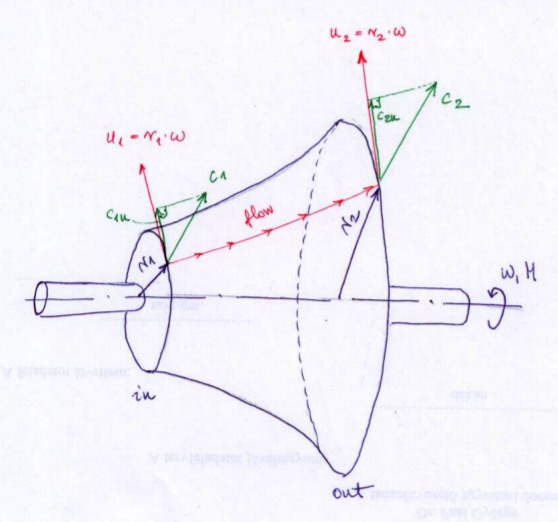
\includegraphics[scale=0.5]{figs/euler_turbine_equation_fig.png}
\caption{\label{gen_turbom}Generalized turbomachine}
\end{center}
\end{figure}

{\bf Derivation 1: Moment of momentum}

Let us compute the moment of the force that is applied at the inlet and outlet of the generalized turbomachine shown in figure \ref{gen_turbom}:

\begin{equation}
\uvec{F}=\frac{\mathrm{d}}{\mathrm{d} t}\left( m \uvec{c}\right)
\quad \rightarrow\quad
\uvec{M}=\frac{\mathrm{d}}{\mathrm{d} t}\left( \uvec{r} \times m \uvec{c}\right)=\dot{m}\left( \uvec{r} \times \uvec{c}\right)
\end{equation}

where $m$ is the mass flow, and $\underline{c}$ is the velocity of the fluid on the radius $r$. We consider the following assumptions:
\begin{itemize}
  \item The inlet of the turbomachine is a circle with radius $r_1$, and the outlet with radius $r_2$.
  \item $\underline{c}$ velocity is considered constant in the sense that its length and angle are constant.
\end{itemize}
Thus $$ \uvec{M} = \uvec{M}_{out}-\uvec{M}_{in}=\dot{m}\left( \uvec{r}_2 \times \uvec{c}_2\right) - \dot{m}\left( \uvec{r}_1 \times \uvec{c}_1\right) $$.
With this the power need of driving the machine is
%
\begin{eqnarray}
	\dot m Y &= & P = \uvec{\omega} \uvec{M} = \left(\uvec{M}_{out}-\uvec{M}_{in}\right)\, \uvec{\omega}
	=\dot m \left[ \uvec{\omega} \left( \uvec{r}_2 \times \uvec{c}_2\right) - \uvec{\omega} \left( \uvec{r}_1 \times \uvec{c}_1\right) \right] \nonumber\\
	&=&\dot m \left[ \uvec{c}_2 \left( \uvec{\omega} \times \uvec{r}_2 \right) - \uvec{c}_1 \left( \uvec{\omega} \times \uvec{r}_1 \right) \right]
	=\dot m \left[ \uvec{c}_2 \uvec{u}_2 - \uvec{c}_1 \uvec{u}_1 \right] \nonumber\\
	&=&\dot m \left[ |\uvec{c}_2| |\uvec{u}_2| - |\uvec{c}_1| |\uvec{u}_1| \right]
	=\dot m \left( c_{2u} u_2 - c_{1u} u_1\right)
\end{eqnarray}
%
where $u_i = |\uvec{u}_i|$, and $c_i=|\uvec{c}_{2u}| cos(\alpha)$.
Comparing the beginning and the end of the equation, we see that the specific work is
\begin{equation}
\boxed{Y=c_{2u} u_2 - c_{1u} u_1}.
\end{equation}

{\bf Derivation 2: Rotating frame and reference and rothalpy}

The Bernoulli equation in a rotating frame of reference reads
%
\beq
\frac{p}{\rho}+\frac{w^2}{2}+U = \mathrm{const.},
\eeq
%
where $U$ is the potential associated with the conservative force field, which is the potential of a rotating frame for reference: $U=-r^2\omega^2/2$. Let $w$ stand for the relative velocity, $c$ for the absolute velocity and $u=r \omega$ for the 'transport' velocity. We have $\uvec{c}=\uvec{u}+\uvec{w}$, thus $w^2=u^2+c^2-2u\,c=u^2+c^2-2u\,c_u$, which gives
\begin{equation}
\frac{p}{\rho}+\frac{w^2}{2}-\frac{r^2 \omega^2}{2}=\frac{p}{\rho}+\frac{c^2+u^2-2c u}{2}-\frac{u^2}{2}=\frac{p}{\rho}+\frac{c^2}{2}-\underbrace{c\,u}_{c_u u}=\mathrm{const}.
\end{equation}

Thus we see that the above quantity is conserved in a rotating frame of reference, which we refer to as \emph{rothalpy} (abbreviation of rotational enthalpy). Let us find now the change of energy inside the machine:
%
\begin{equation}
Y=\Delta \left(\frac{p}{\rho}+\frac{c^2}{2}\right)=\Delta \left( c_u u\right),
\end{equation}
%
which is exactly Euler's turbine equation. (For compressible fluids, rothalpy is $I=c_p T+\frac{c^2}{2}-u c_{u}$.)

\section{Velocity triangles and performance curves} \label{sec:velocity_triangles_pumps}

% \begin{figure}[ht]
% 	\begin{center}\label{fig:velcoitytriangles}
% 		%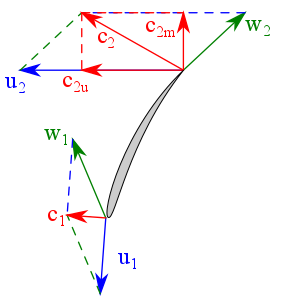
\includegraphics[scale=0.5]{figs/VelocityTriangles.png}
% 		%\includegraphics[scale=0.5]{Impeller3D_and_VelocityTriangles_v2.png}
% 		\includegraphics[width=0.8\textwidth]{Impeller2D_and_VelocityTriangles.png}
% 		\caption{Velocity triangles at the inlet and at the outlet}
% 	\end{center}
% \end{figure}

% \note{VelocityTriangle figure added by Weber Richard}
From the Euler turbine equation we have:
%
\begin{equation*}
  \Delta p_e = \rho g H = \rho \left( c_{2u}u_2 - c_{1u}u_1 \right)
\end{equation*}
%
where $H$ is the head of the pump. Known the velocity triangle's components and the density of the fluid, we get:
%
\begin{equation}\label{radial_head}
  H = \frac{c_{2u}u_2 - c_{1u}u_1}{g}
\end{equation}
%
The volume flow rate is
\begin{equation}\label{radial_flow}
  Q = c_{2m} A_2 =c_{2m} D_2 \pi b_2,
\end{equation}
%
where $D_2$ is the impeller outer diameter, $b_2$ is its flow-through width at the outlet. From \ref{radial_head} and \ref{radial_flow} we have that $\uvec{c}$ outlet absolute velocity is the connection between the head and the flow rate of the pump. Also one can notice, that if $ \Delta p_e$ increased, that is when $c_{2u}$ is increased than $Q$ decreases ($c_{2m}$ decreases). And if $\Delta p_e$ decreased ($c_{2u}$ decreased) than $Q$ increases ($c_{2m}$ increases). So our goal now is to find a relationship between the head and the flow rate of the pump.

\subsection{Radial (centrifugal) machines}

Let us consider a centrifugal pump and the velocity triangles at the impeller inlet and outlet, see Fig. \ref{fig:centrifual_pumps}. The theoretical volume flow rate is
%
\begin{equation}
Q_{th}=c_{2m} A_2 \Psi =c_{2m} D_2 \pi b_2 \Psi,
\end{equation}
%
where $D_2$ is the impeller outer diameter, $b_2$ is its flow-through width at the outlet and $c_{2m}$ is the radial component of the outlet absolute velocity. $\Psi<1$ is a constant called \emph{blockage factor} that takes into account that the real flow through area is smaller due to the blockage of the blade width at the outlet.

\begin{figure}[ht]
\begin{center}
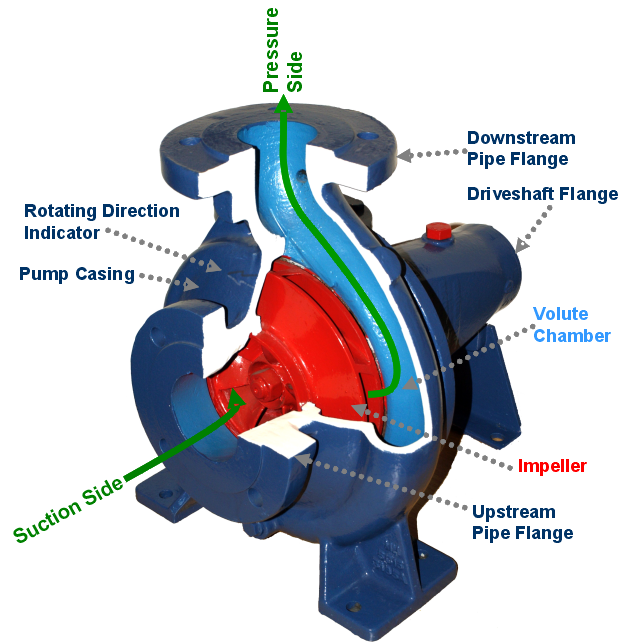
\includegraphics[width=0.52\textwidth]{figs/Centrifugal_Pump.png}
%\includegraphics[width=0.45\textwidth]{figs/Double-Suction-Centrifugal-Pump.jpg}
\caption{\label{fig:centrifual_pumps}Centrifugal pumps}
\end{center}
\end{figure}

%\begin{minipage}{\textwidth}

%\begin{floatingfigure}[r]{0.5\textwidth}
%\begin{center}
%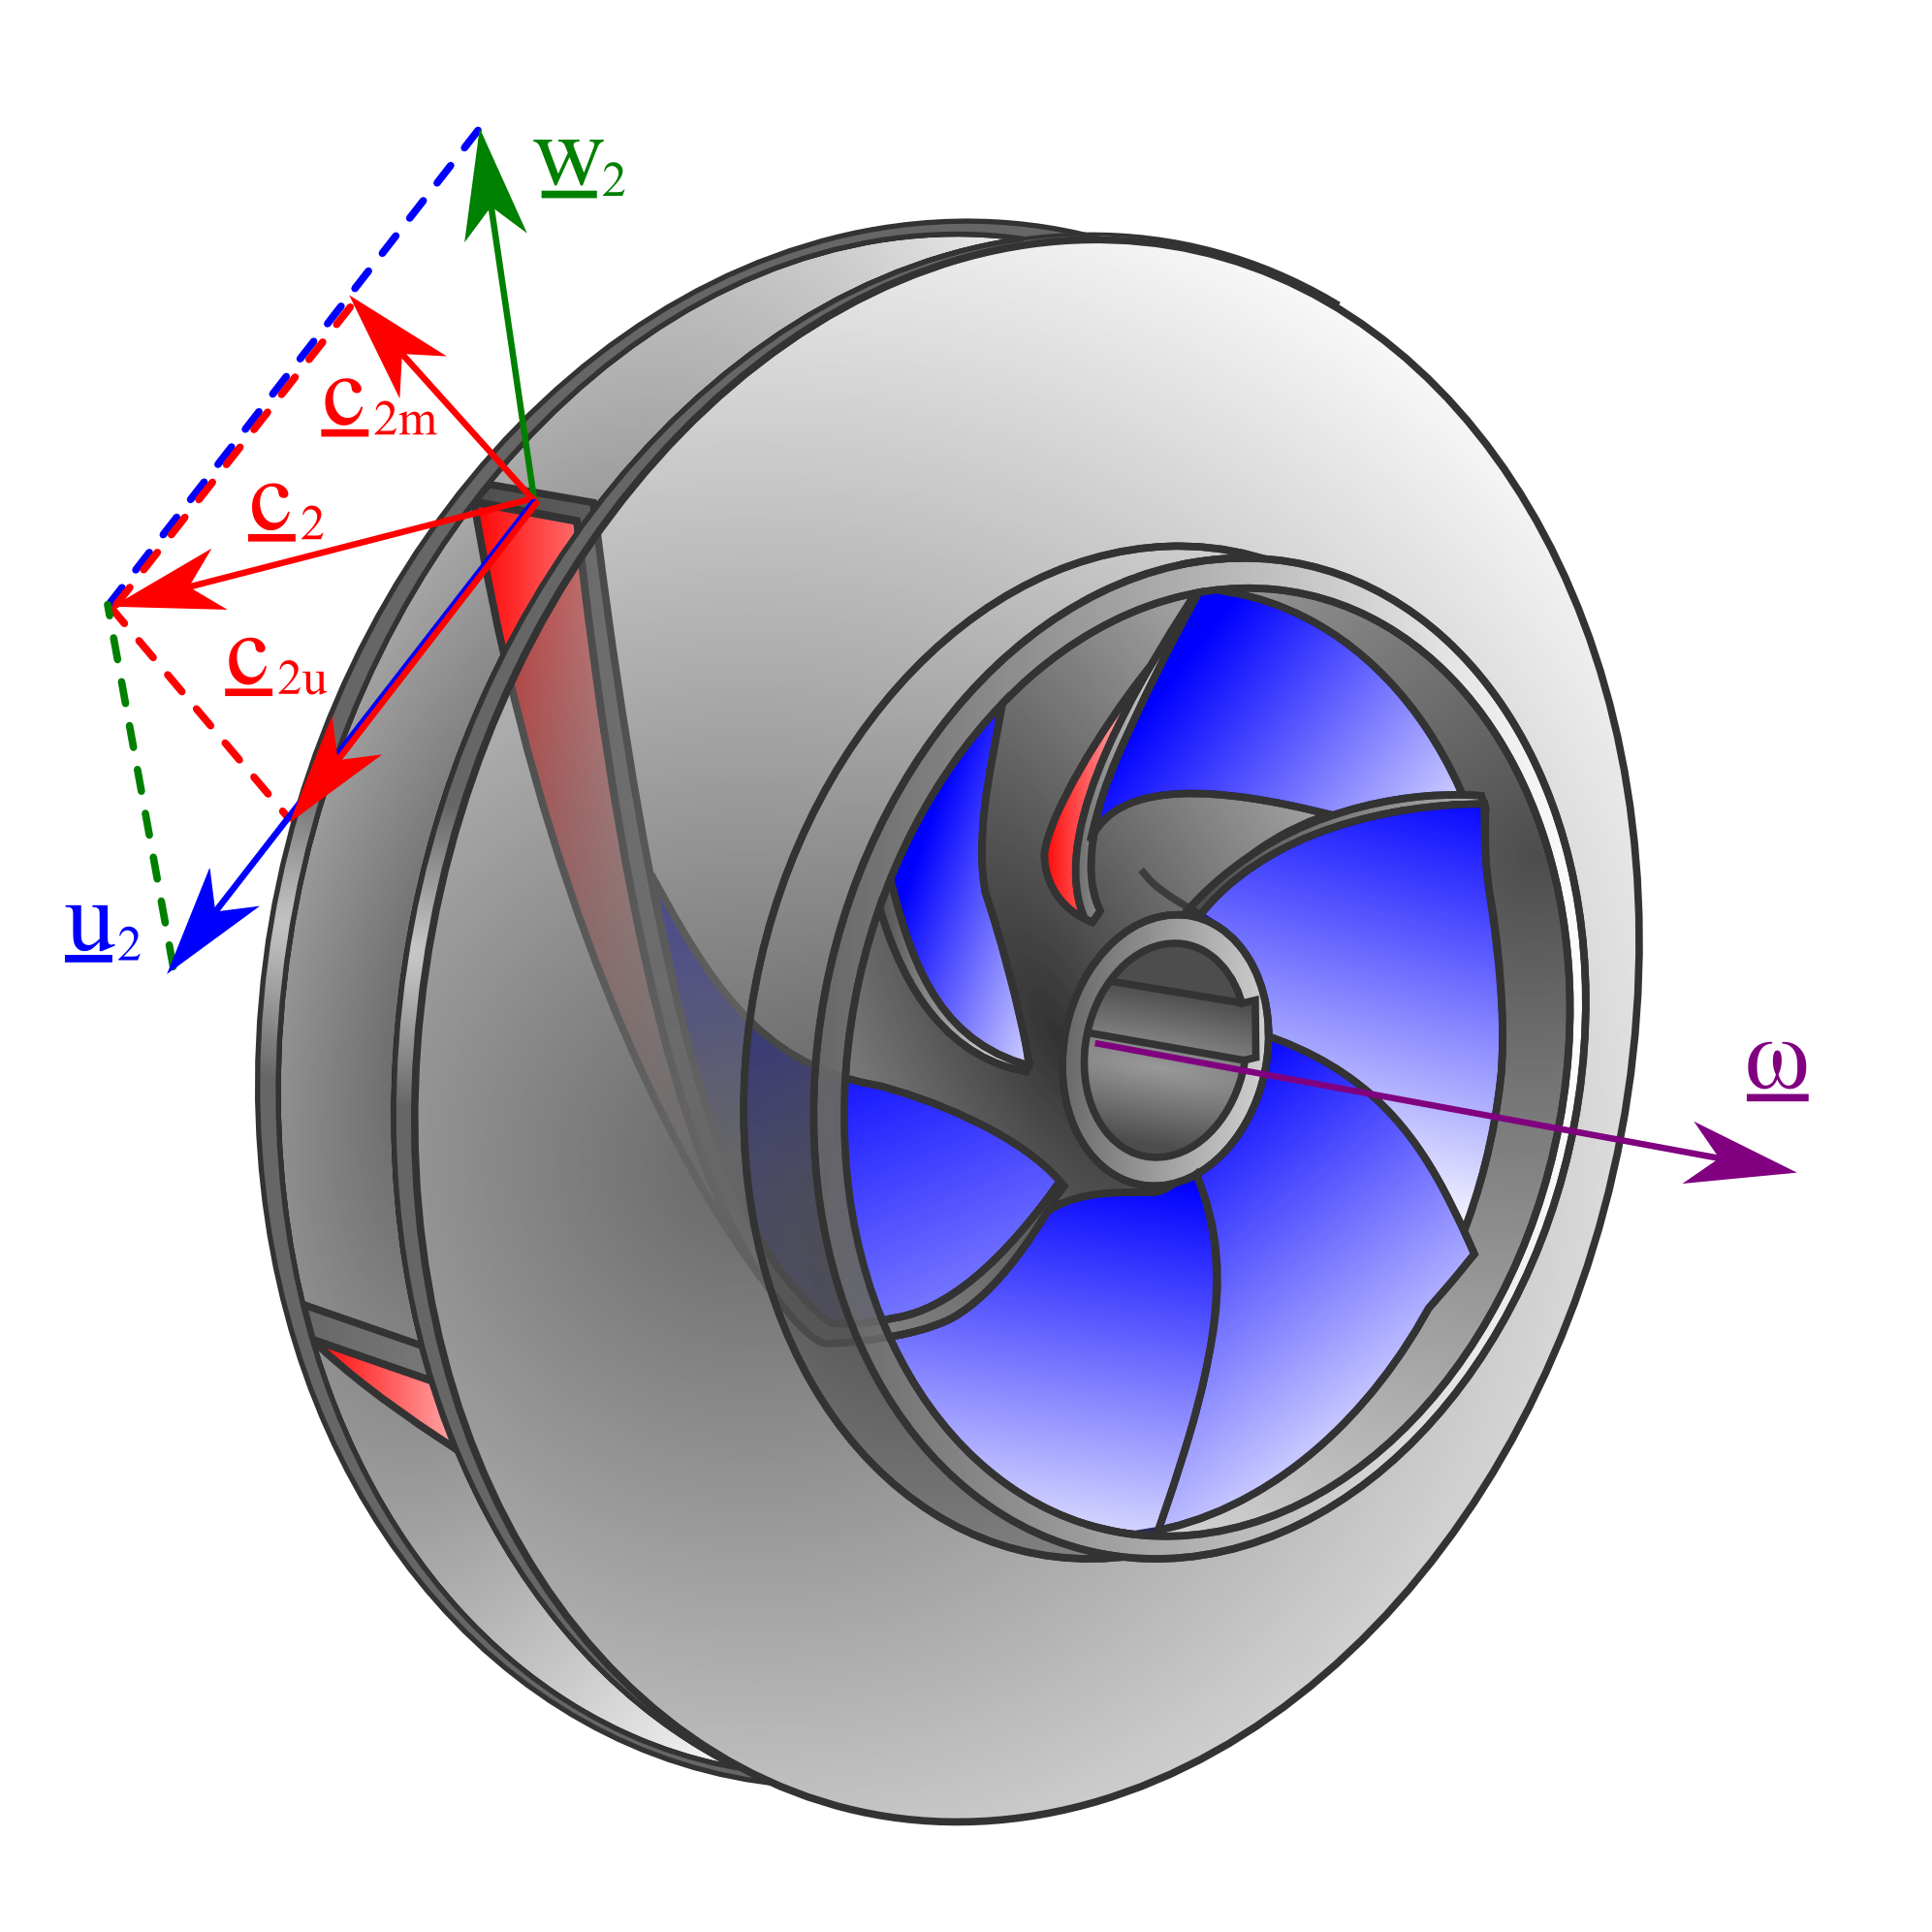
\includegraphics[width=0.35\textwidth]{figs/Impeller3D_and_VelocityTriangles.png}
%\caption{\label{fig:centrifual_pumps_velocity_triangle}Centrifugal impeller with outlet velocity components.}
%\end{center}
%\end{floatingfigure}

\begin{figure}[ht]
\begin{center}
\includegraphics[width=6cm]{figs/Impeller3D_and_VelocityTriangles_v2.png}
\hspace{0.5cm}
\includegraphics[width=7.5cm]{figs/Impeller2D_and_VelocityTriangles.png}
\caption{\label{fig:centrifual_pumps_velocity_triangle}Centrifugal impeller with outlet velocity components.}
\end{center}
\end{figure}

The velocity triangle describes the relationship between the absolute velocity $c$, the circumferential velocity $u$ and the relative velocity $w$. Obviously, we have $\vec{c}=\vec{u}+\vec{w}$. Moreover, we know that (a) the circumferential velocity is $u=D \pi n$ and that (b) the relative velocity is tangent to the blade, i.e. the angle between $u$ and $w$ is approximately the blade angle $\beta$.

Basic trigonometrical identities show that $c_{2u}=u_2-c_{2m}/\tan \beta_2$. It is usual to assume that the flow has no swirling (circumferential) component at the inlet (due to Helmholtz's third theorem). In the reality, the outlet flow angle is not exactly $\beta_2$, thus the head is decreased, which is taken into account with the help of the \emph{slip factor} $\lambda$ (sometimes denoted by $\sigma$ in the literature).
%\end{minipage}

If there is no \emph{prerotation} (i.e. $c_{1u}=0$), we have
%
\begin{align}
H_{th}&=\lambda \frac{c_{2u} u_2}{g}=\lambda\left(\frac{u_2^2}{g}-\frac{u_2}{g}\frac{w_{2u}}{g}\right)=\lambda\left(\frac{u_2^2}{g}-\frac{u_2}{g}\frac{c_{2m}}{\tan \beta_2}\right)\nonumber \\
&=\lambda\left(\frac{u_2^2}{g}-\frac{u_2}{g\tan \beta_2 D_2 \pi b_2 \Psi}Q_{th}\right).
\end{align}

Thus, the theoretical performance curve $H_{th}(Q_{th})$ of a centrifugal machine is a straight line, which is (see Figure \ref{fig:blade_shapes})
\begin{itemize}
\item decreasing as $Q$ is increased, for \emph{backward curved} blades, i.e. $\beta_2<90^o$,
\item horizontal, for \emph{radial blades} ($\beta_2=90^o$) and
\item increasing (as $Q$ is increased) for \emph{forward curved} blades, i.e. $\beta_2>90^o$.
\end{itemize}

\begin{figure}[ht]
\begin{center}
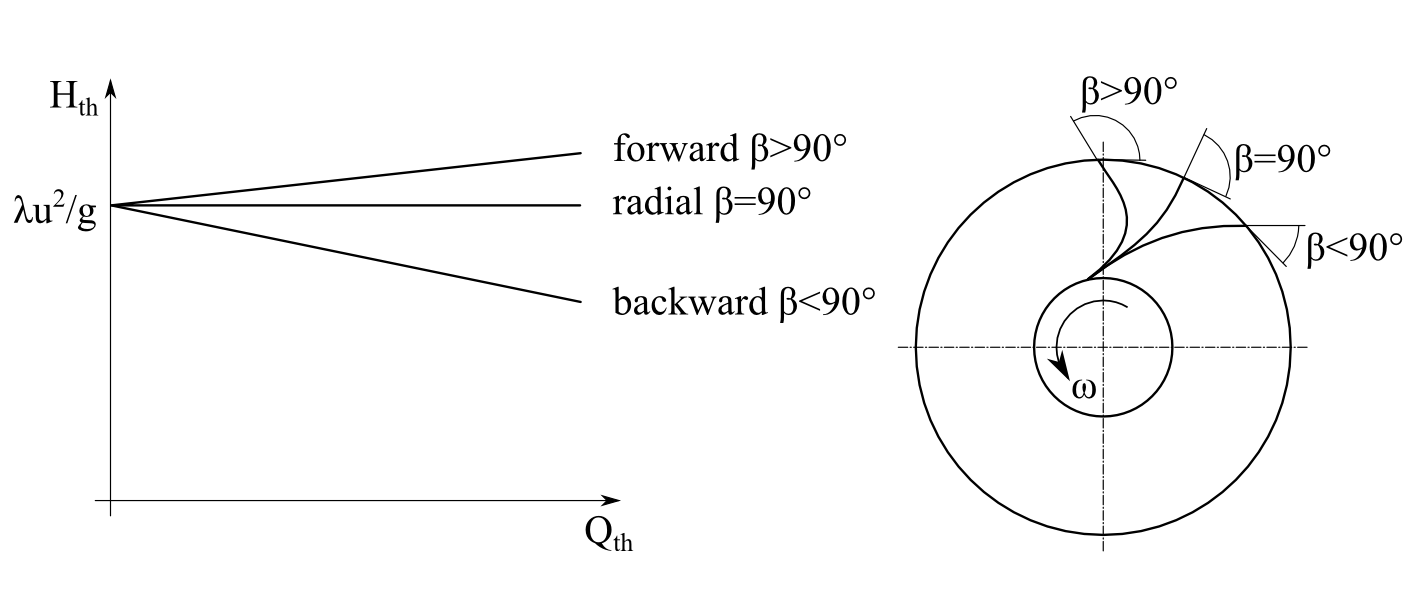
\includegraphics[width=0.8\textwidth]{figs/RadialPump_BladeShapes.png}
\caption{\label{fig:blade_shapes}Effect of blade shapes $\beta_2$ angle on the performance curve.}
\end{center}
\end{figure}

\subsection{Problems}

\noindent {\bf Problem \thesection.\theprob}\stepcounter{prob} 

A radial impeller runs at n=1440/min revolution speed and conveys $Q=40$ l/s of water. The diameter of the impeller is $D= 240$ mm, the outlet width is $b_2=20$ mm. The blade angle at the outlet is $\beta_2 = 25$ degrees. The inlet is prerotation-free. Find the theoretical head and draw a qualitatively proper sketch of the velocity triangle at the outlet. (Solution: $H_{th}=22.9$m)

\vspace{1cm}
\noindent {\bf Problem \thesection.\theprob}\stepcounter{prob}

The mean meridian velocity component of a radial impeller with $D_2=400$ mm diameter at $n=1440$rpm revolution speed is $c_m= 2.5$ m/s. The angle between the relative and circumferential velocity components is $\beta_2=25$ degrees. With a geometrical change of the blade shape, this angle is increased to to 28 degrees, that results in 10\% drop of the meridian velocity component. The inlet is prerotation-free. Find the relative head change. (Solution: $(H_{25^o}-H_{28^o})/H_{25^o}=4.6$\%) 



\subsection{Axial machines}

In the case of axial machines the flow leaves the impeller axially, see Fig. \ref{fig:axial_pumps}. The flow-through area is $\left(D_o^2-D_i^2\right)\pi/4$, where $D_o$ and $D_i$ stand for the outer and inner diameter of the lade, respectively. Notice that in this case, $u_1=u_2$ because it is assumed that the flow moves along a constant radius. Assuming (again) prerotation-free inlet ($c_{1u}=0$), we have $c_{2m}=c_1$ (due to continuity).

\begin{figure}[ht]
\begin{center}
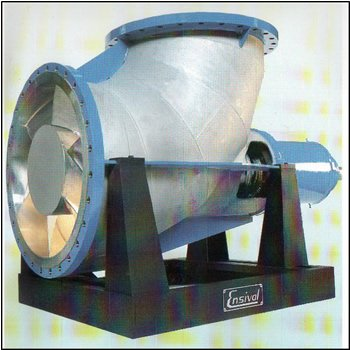
\includegraphics[width=0.3\textwidth]{figs/axial_pump1.jpg}
\hspace{1cm}
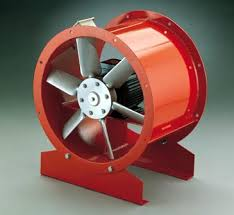
\includegraphics[width=0.3\textwidth]{figs/axialfanplate.jpg}
\caption{\label{fig:axial_pumps}Axial pump (left) and axial fan (right)}
\end{center}
\end{figure}

However, an important difference between axial and centrifugal pumps (fans) is that in the case of axial machines, the pressure rise changes along the radial coordinate of the blade:
%
\beq
\Delta p_t(r)=\left.\rho u(r) \left(c_{2u}(r)-c_{1u}(r) \right)\right|_{c_{1u}=0}=\rho \left( 2 r \pi n \right) \left(2 r \pi n-\frac{c_{2m}}{\tan \beta_2} \right).
\eeq
%
Thus, if we wanted to obtain \emph{constant} $\Delta p_t$ along the radial coordinate, the change of the circumferential velocity has to be compensated by varying $\beta_2$.

\begin{figure}[ht]
\begin{center}
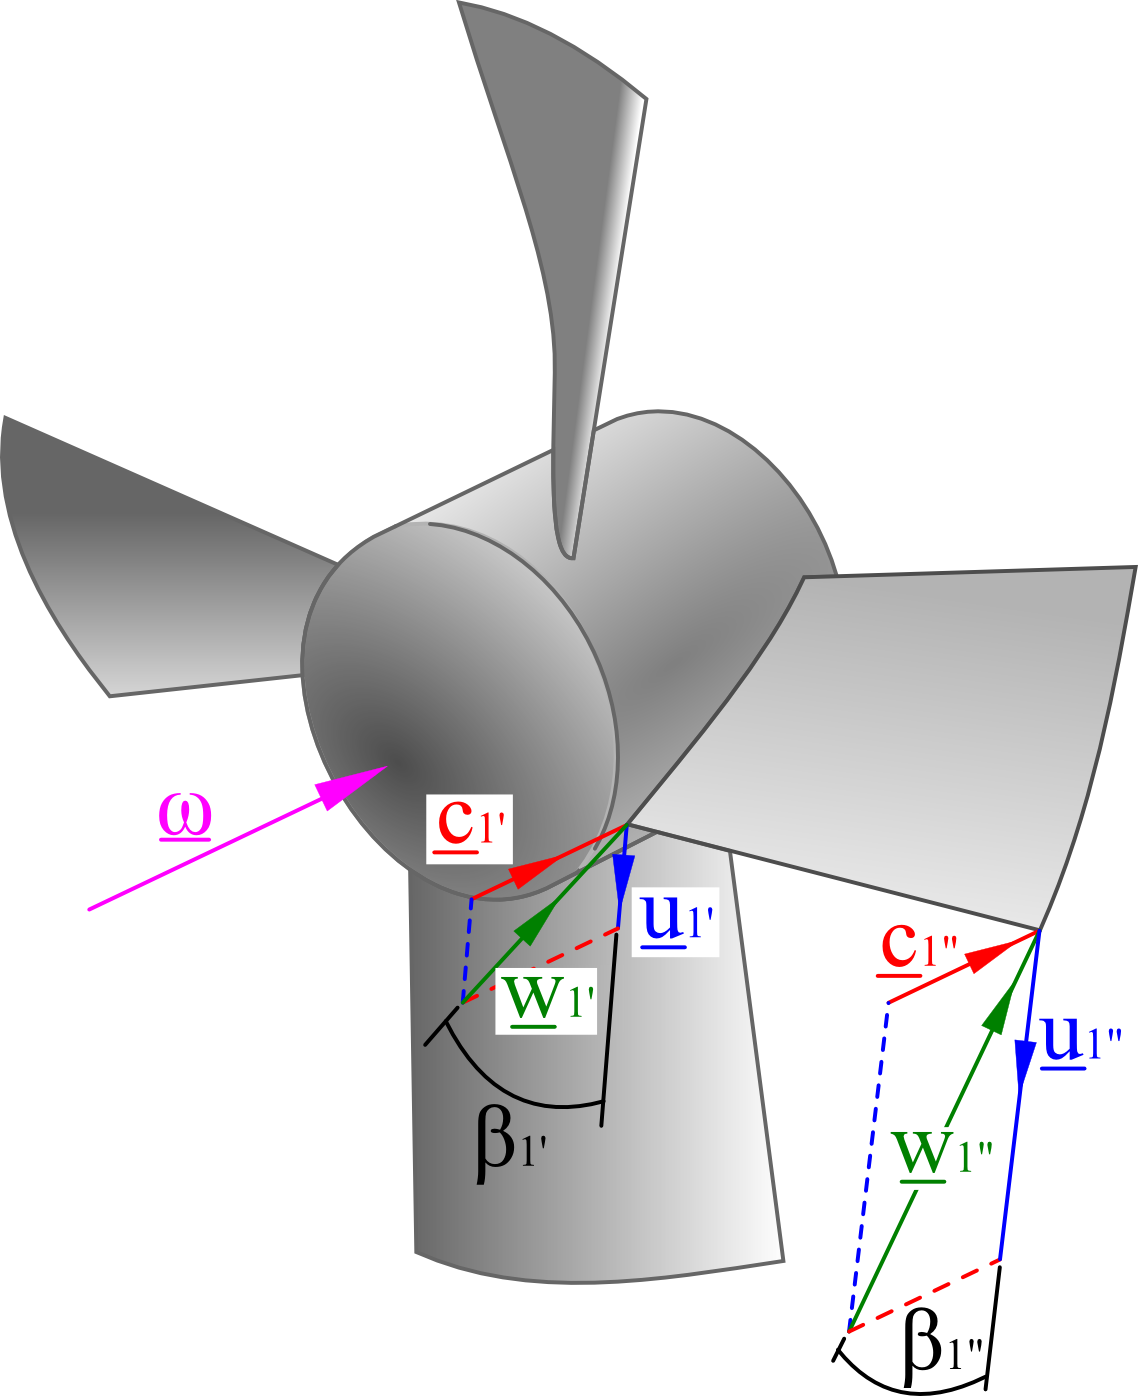
\includegraphics[width=0.3\textwidth]{figs/AxialPump_axon.png}
\hspace{1cm}
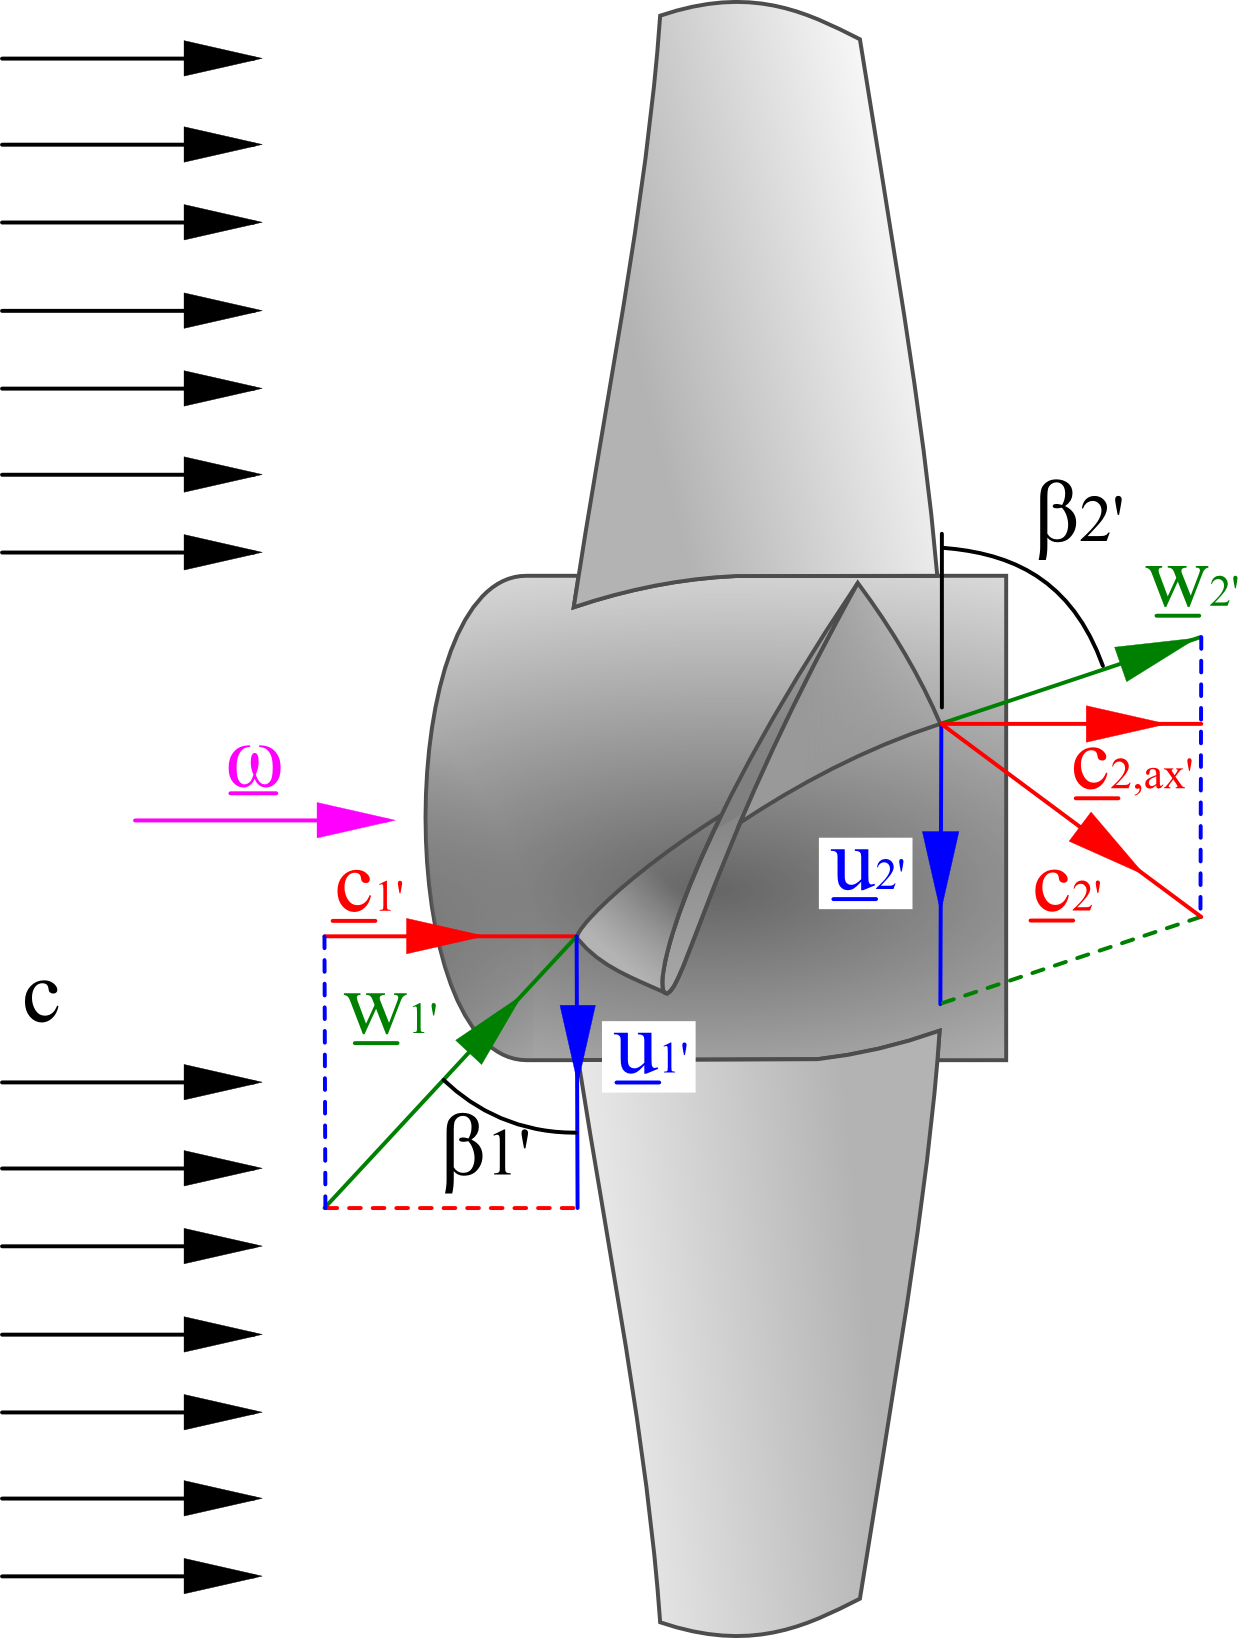
\includegraphics[width=0.3\textwidth]{figs/AxialPump_side.png}
\caption{\label{fig:axial_machines}Axial impeller with outlet velocity components.}
\end{center}
\end{figure}

%\begin{minipage}{\textwidth}
%
%\begin{floatingfigure}[r]{0.5\textwidth}
%\centering
%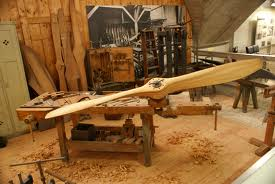
\includegraphics[width=0.45\textwidth]{figs/WorldWarWoodenPropeller.jpg}
%\caption{\label{fig:propeller}World War I wooden propeller}
%\end{floatingfigure}
%
%The twisted airfoil (aerofoil) shape of modern aircraft propellers was pioneered by the Wright brothers. While both the blade element theory and the momentum theory had their supporters, the Wright brothers were able to combine both theories. They found that a propeller is essentially the same as a wing and so were able to use data collected from their earlier wind tunnel experiments on wings. They also found that the relative angle of attack from the forward movement of the aircraft was different for all points along the length of the blade, thus it was necessary to introduce a twist along its length. Their original propeller blades are only about 5\% less efficient than the modern equivalent, some 100 years later. (Source: Wikipedia)
%
%\end{minipage}

\subsection{Problems}
\begin{tcolorbox}
\noindent {\bf Problem \thesection.\theprob}\stepcounter{prob}

The outer diameter of a CPU axial cooler ventilator is $D_o=47\,\mathrm{mm}$ the inner diameter is $D_i=21.5\,\mathrm{mm}$ the revolution speed is $n=2740\,\mathrm{rpm}$. Due to the careful design the hydraulic efficiency is $\eta_h=85\%$ however the volumetric efficiency as consequence of leakage flow rate between the housing and the impeller is just $\eta_{vol}=75\%$. The blade angle at the suction side is $\beta_1=20^\circ$ while at the pressure side $\beta_2=40^\circ$. Find the flow rate and the total pressure rise on the impeller. The density of the air is $\rho=1.25\,\mathrm{kg/m^3}$. Draw the velocity triangles at the inlet and the outlet at the mean diameter.
%
\begin{itemize}
\item $A_{ring}=\frac{\left(D_o^2-D_i^2\right)\pi}{4}=0.00137\,\mathrm{m^2}$
\item $D_{mean}=\frac{D_o+D_i}{2}=0.03425\,\mathrm{m}$
\item $u_{mean}=u_1=u_2=D_{mean}\pi n=4.913\,\mathrm{\frac{m}{s}}$
\item $c_{ax}=c_{1,ax}=c_{2,ax}=u \tan\beta_1=1.788\,\mathrm{\frac{m}{s}}$
\item $q=\eta_{vol}A_{ring}c_{ax}=0.00184\,\mathrm{\frac{m^3}{s}}$
\item $w_{2u}=\frac{c_{ax}}{\tan\beta_2}=2.131\,\mathrm{\frac{m}{s}}$
\item $\Delta c_u=u-w_{2u}=2.782\,\mathrm{\frac{m}{s}}$
\item $\Delta p_{total,ideal}=\rho u\Delta c_u=17.1\,\mathrm{Pa}$
\item $\Delta p_{total}=\eta_h \Delta p_{total,ideal}=14.5\,\mathrm{Pa}$
\end{itemize}
\end{tcolorbox}
	
\vspace{1cm}
\begin{tcolorbox}
\noindent {\bf Problem \thesection.\theprob}\stepcounter{prob}

The inner diameter of an axial impeller is $D_i=250$ mm, while the outer one is $D_o=400$mm. The revolution number of the impeller is $1470$rpm. The inlet is prerotation-free. At $Q=0.36\,\mathrm{ m^3/s}$ the hydraulic efficiency is 85\%, the head is 6 m. The specific work along the radius is constant. Find the angles $\beta_{1,2}$  at the inner and outer diameter. 


%(Solution: $\beta_{1,i}=13.7$, $\beta_{2,i}=16.7$, $\beta_{1,o}=8.7$ and $\beta_{2,o}=9.4$ degrees) 
\vspace{0.2cm}

Solution:

\begin{itemize}
%
\item The velocity triangles are depicted in the Figure \ref{gen_vtr}.
%
\item The circumferential speed at the inner diameter is $u_{2i}=D_i\pi n=0.25\pi \frac{1470}{60}= 19.24 m/s$. The two circumferential speeds $u_{i,1}$ and $u_{i,2}$ equal as they are located at the same (inner) radius.
%
\item The circumferential speed at the outer diameter is $u_{20}=D_o\pi n=0.4\pi\frac{1470}{60}= 30.79 m/s$. Again the the two circumferential speeds $u_{o,1}$ and $u_{o,2}$ equal as they are located at the same (outer) radius.
%
\item The theoretical head is $H_{th}=\frac{c_{2u}u_2}{g}=\frac{H}{\eta_h}=7.059m$. We also have  $c_{2u}u_2=H_{th}g=69.247$ $m^2/s^2$, which is constant along the radius: $c_{2u,i}=\frac{69.247}{19.24}=3.56$ m/s and $c_{2u,o}=\frac{69.247}{30.79}=2.25$ m/s.
%
\item The axial component of the velocity is $c_{ax}=\frac{4Q}{\left({D_o}^2-{D_i}^2\right)\pi}=\frac{4 \times 0.36}{\left({0.4}^2-{0.25}^2\right)\pi}=4.70$ m/s
%
\item The blade angles are
\begin{equation*}
\beta_{1i}=\arctan\frac{c_{ax}}{u_{2i}}=
%=\arctan\frac{4.70}{19.24}=
13.73^o \quad \text{and}\quad \beta_{2i}=\arctan\frac{c_{ax}}{u_{2a}-c_{2ui}}
%=arctan\frac{4.70}{19.24-3.56}=
=16.7^o.
\end{equation*}

\item With the same train of thought, one obtains $\beta_{10}=8.7^o$ and $\beta_{20}=9.4^o$.
\end{itemize}
\end{tcolorbox}
\vspace{1cm}

\begin{figure}[ht]
\begin{center}
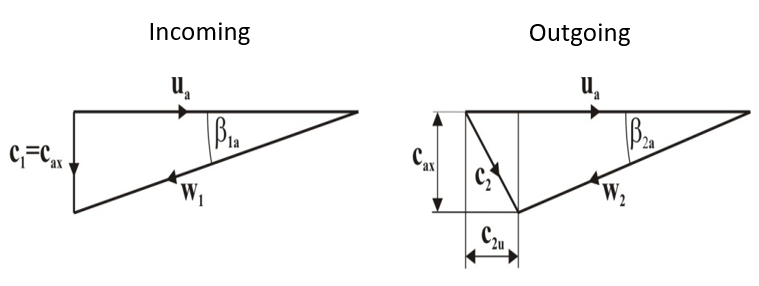
\includegraphics[scale=0.6]{figs/problem_2p2p16_vel_tri_fig.png}
\caption{\label{gen_vtr}Velocity triangles}
\end{center}
\end{figure}



\clearpage

\subsection{Real performance curves} \label{sec:real_performance_curves_turbomachines}

Our analysis so far assumed that the flow inside the impeller is ideal (no losses) and that the streamlines are following the blade shape (thus, blade angles are also the streamline angles). However neither of these assumptions are true.

There are significant friction losses inside the impeller, the narrower the flow passage is, the higher the friction losses will be. Moreover, the volute also introduces friction losses. These losses are proportional to the velocity squared, thus $H'_{friction} \propto Q^2$.

On the other hand, if the angle of attack deviates from the ideal one, one experiences separation on the two sides of the blade. This is illustrated in Figure~\ref{fig:real_perf_curve} for a constant circumferential velocity $u$ as the flow rate and thus the inlet velocity $c$ is varied, the relative velocity $w$ also varies. At the design flow rate $Q_d$ the angle of attack ideal. For small flow rates, we have separation on the suction side of the blade, while for larger flow rates the separation is on the pressure side of the blade. Thus we have $H'_{separation} \propto (Q-Q_d)^2$.

To obtain the real performance curve, one has to subtract the above two losses from the theoretical head: $H=H_{th}(Q)-K_1 Q^2-K_2 (Q-Q_d)^2$, which is illustrated in \ref{fig:real_perf_curve}. Note that at the design point and close to it, the friction losses are moderate and no separation occurs. For lower flow rates, the friction loss decreases while separation increases. For higher flow rates, both friction and separation losses increase.

\begin{figure}[ht]
\centering
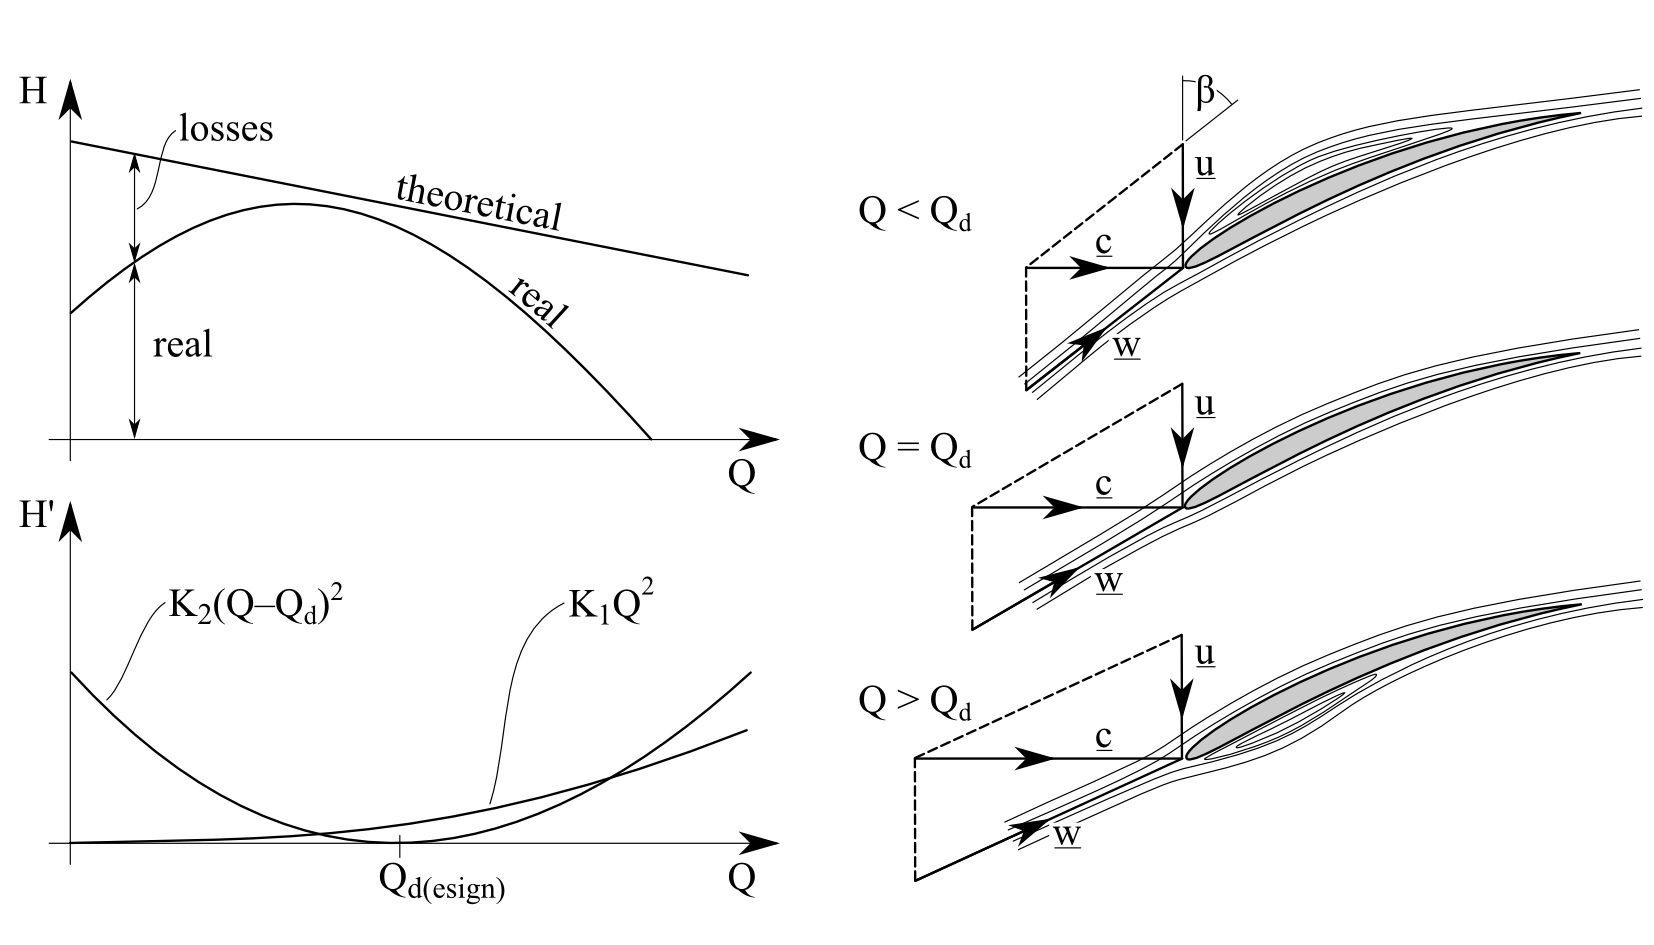
\includegraphics{figs/HeadLosses.png}
\caption{\label{fig:real_perf_curve}Friction and separation losses in the impeller.}
\end{figure}

%%%%%%%%%%%%%%%%%%%%%%%%%%%%%%%%%%%%%%%%%%%%%%%%%%%%%%%%%%%%%%%%%%%%%%%%%%%%%%%%%%%%%%%%%%%%%%%

\clearpage

\section{Losses and efficiencies}

Let us analyse the losses that decrease the efficiency of a turbomachine (see Figure~\ref{fig:PumpLosses}).

\begin{figure}[ht]
\centering
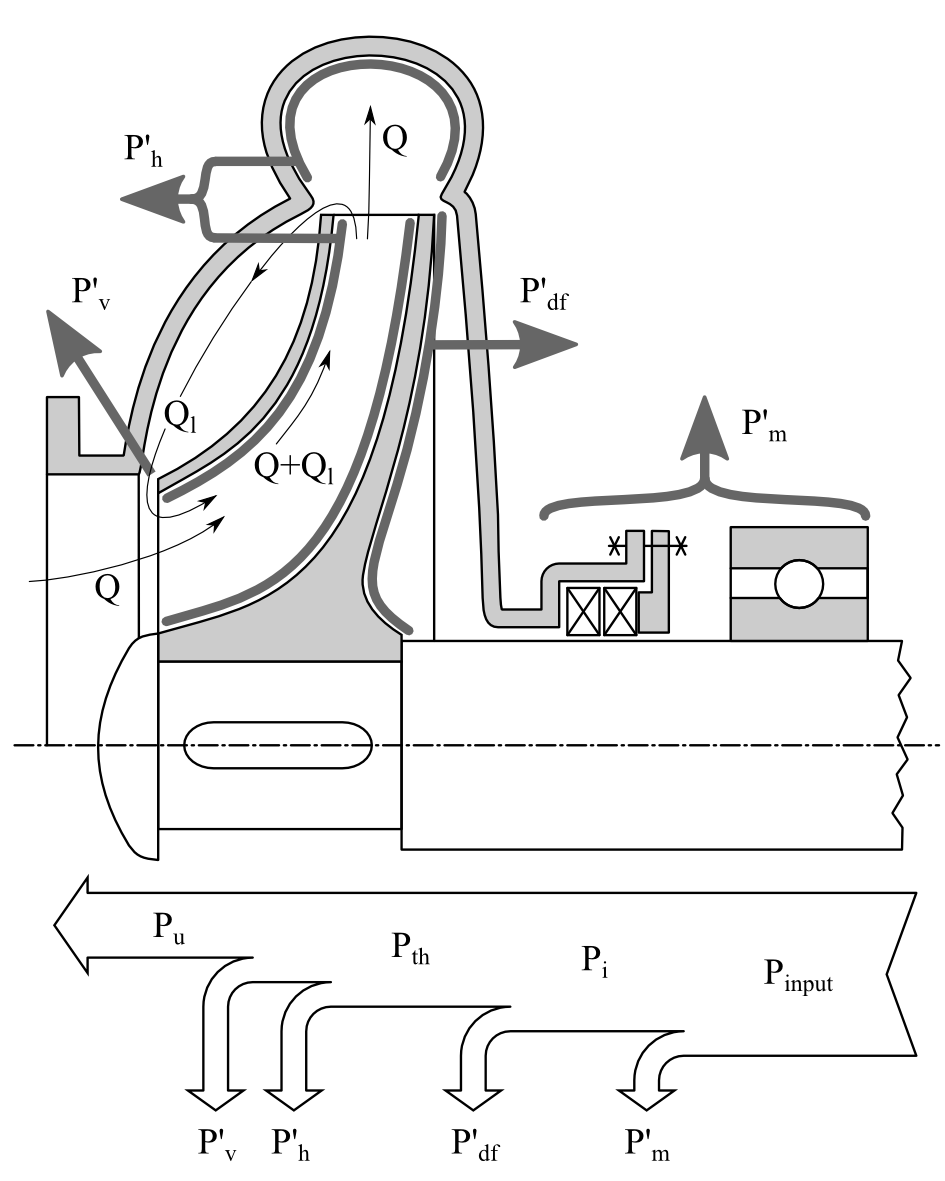
\includegraphics{figs/PumpLosses.png}
\caption{\label{fig:PumpLosses}Losses of the pump.}
\end{figure}

\noindent Let the input mechanical power transmitted by the shaft be denoted by $P_{input}$. We have than

\begin{description}
\item[Mechanical losses $P'_m$] These represent the friction loss in the bearings and the mechanical sealing losses (if any). The remaining power is called \emph{internal power} $P_i=P_{input}-P'_m$.
%
\item[Disc friction losses $P'_{df}$] A significant shear force appears in the fluid entrapped between the housing and the impeller, which is taken into account by the \emph{disc friction coefficient}: $P'_{df}=\nu_{df} P_i$. The remaining power is the theoretical power of the impeller: $P_{th}=P_i-P'_{df}=(1-\nu_{df}) P_i$.
%
\item[Hydraulic and volumetric losses $P'_h$, $P'_v$] The theoretical head $H_{th}$ and flow rate $Q_{th}$ and is further decreased by the leakage flow rates ($Q_{l(eakage)}$) inside the pump (flow across the gaps between the impeller and the housing) and the internal frictional losses $h'$ (e.g. in the impeller and volute). We have
\begin{align}
P_{th}&=Q_{th} \rho g H_{th}=\left( Q+Q_{l}\right) \rho g \left( H+h'\right)=\underbrace{Q \rho g H}_{P_{u}}+\underbrace{Q_l \rho g H}_{P'_v}+\underbrace{Q_{th}\rho g h'}_{P'_h}\nonumber\\
&=Q\rho g H \frac{Q+Q_{l}}{Q}\frac{H+h'}{H}=Q\rho g H \underbrace{\frac{Q_{th}}{Q}}_{\eta_v^{-1}} \underbrace{\frac{H_{th}}{H}}_{\eta_h^{-1}} \quad \rightarrow \quad P_u=P_{th}\eta_h \eta_v
\end{align}
\end{description}

\newpage
\subsection{Problems}


\begin{tcolorbox}
\noindent {\bf Problem \thesection.\theprob}\stepcounter{prob}

The revolution number of a water pump is 1470 rpm, the flow rate is $Q=0.055\mathrm{m^3/s}$ and the head is $H=45$m. The hydraulic power loss is $P'_h=2.5$kW, the mechanical power loss is $P'_m=1.3$kW, the disc friction coefficient is $\nu_t=0.065$. The input power at this operating point is $P_{in}=32$kW. Make a complete analysis of the losses, including leakage flow rate and the theoretical head.

\noindent Solution:

The power flow chart is in Figure \ref{gen_pfc}

\begin{itemize}
\item $P_{i}=P_{input}-P'_{m}=30.7\,\mathrm{kW}\quad \rightarrow \quad \eta_{m}=95.9\%$
\item $P_{th}=(1-\nu)P_{i}=28.7\,\mathrm{kW}$
\item $h'_{h}=\frac{P'_{h}}{\rho g Q}=4.63\,\mathrm{m} \quad \rightarrow \quad H_{th}=45+4.63=49.63\,\mathrm{m}\quad \rightarrow \quad \eta_{hydr}=90.6\%$
\item $Q_{th}=\frac{P_{th}}{\rho g H_{th}}=0.0589\,\mathrm{m^3/s}\quad \rightarrow \quad Q_{leakage}=0.00395\,\mathrm{m^3/s}\quad \rightarrow \quad \eta_{v}=93.2\%$ 
\item $\eta_{overall}=\eta_{v} \cdot\eta_{h} \cdot (1-\nu) \cdot \eta_{m} = 75.9\%$
\end{itemize}
\end{tcolorbox}
\vspace{1cm}

\begin{figure}[ht]
\begin{center}
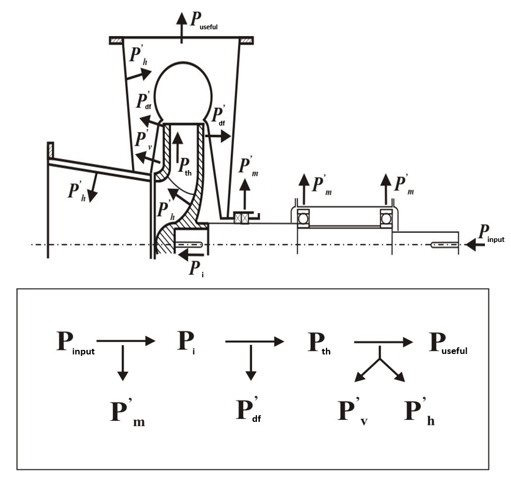
\includegraphics[scale=0.85]{figs/problem_2p3p17_pow_flow_chart_fig.png}
\caption{\label{gen_pfc}Power flow chart}
\end{center}
\end{figure}

\vspace{1cm}
\noindent {\bf Problem \thesection.\theprob}\stepcounter{prob}

\note{problem added by Weber Richard}
Calculate the theoretical head, the theoretical volume flow rate, the hydraulic efficiency and the volumetric efficiency based on the data of the water pump. $P_{input} = 43.5\,kW,$ $Q = 1100\,dm^3/min,$ $H = 180\,m,$ $P'_{mech} = 1.6\,kW,$ $\nu_{df} = 0.03, h' = 32\,m$.
(Solution: $H_{th} = 212\,m,$ $Q_{th} = 0.01954\,m^3/s$ $\eta_{hydr} = 84.9\%$ $ \eta_{vol} = 93.8\%$)

%----------------------------------------------------------------------------
\clearpage
\section{Dimensionless numbers and affinity} \label{sec:dimensionless_numbers}

Based on the previously obtained formulae for theoretical head, we define dimensionless numbers as
\beq
H=\eta_h H_{th}=2 \eta_h \frac{c_{2u}}{u_2}\frac{u_2^2}{2g}:=\psi \frac{u_2^2}{2g}
\eeq
%
or, in the case of fans
\beq
\Delta p_t=\psi \frac{\rho }{2}u_2^2,
\eeq
%
where $\psi$ is a dimensionless pressure rise. Similarly, we have
%
\beq
Q=\eta_v Q_{th}=\eta_v D_2 \pi b_2 c_{2m}=\eta_v \frac{4 D_2 \pi b_2}{4 D_2^2} \frac{c_{2m}}{u_2} u_2 D_2^2:=\varphi \frac{D_2^2 \pi}{4}u_2
\eeq

These dimensionless quantities are called \emph{pressure number} $\psi$ and \emph{flow number} $\varphi$. What we found is that $H \propto n^2$ and $Q \propto n$ allowing the transformation of the performance curve given at $n_1$ to be computed to another revolution number $n_2$. This is called \emph{affinity law}:
%
\beq
\frac{H_1}{H_2}=\left( \frac{n_1}{n_2}\right)^2, \quad \frac{Q_1}{Q_2}=\frac{n_1}{n_2} \quad \rightarrow \quad \frac{P_1}{P_2}=\left( \frac{n_1}{n_2}\right)^3
\eeq

As we have seen, both $\psi$ and $\varphi$ contains two parameters, $D_2$ and $u_2$, out of which one can be eliminated, resulting in new dimensionless numbers. Let us start with the elimination of $D_2$.
%
\begin{align}
\varphi&=\frac{Q}{\frac{D_2^2 \pi}{4}u_2}=\frac{4 Q}{D_2^3 \pi^2 n}\\
\psi&=\frac{H}{ \frac{u_2^2}{2g}}=\frac{2g H}{ D_2^2 \pi^2 n^2}
\end{align}
%
from which we have
%
\beq
\sigma=\frac{\varphi^{1/2}}{\psi^{3/4}}=\frac{2 \sqrt{Q}}{D_2^{3/2} \pi \sqrt{n}}\frac{ D_2^{3/2} \pi^{3/2} n^{3/2}}{\left(2g H\right)^{3/4}}=\frac{\sqrt{\pi}}{\sqrt[4]{2} g^{3/4}} \underbrace{n \frac{Q^{1/2}}{H^{3/4}}}_{n_q}
\eeq
%
Note that $\sigma$ depends only on the revolution number but takes different values along the performance curve. Thus when actually computing it, one takes the data of the best-efficiency point. Moreover, we do not include the constant term$ \frac{\sqrt{\pi}}{\sqrt[4]{2} g^{3/4}}$. Finally, by definition, the \emph{specific speed} of a turbomachine is

\beq
n_q=n[rpm]\frac{\left(Q_{opt.}[m^3/s]\right)^{1/2}}{\left(H_{opt.}[m]\right)^{3/4}}
\eeq

Specific speed defines the shape of the impeller, low specific speed means low flow rate and high pressure rise (radial impeller) while high specific speed occurs when the flow rate is high and the pressure rise is low, see Fig. \ref{fig:nq}.

\begin{figure}[ht]
\begin{center}
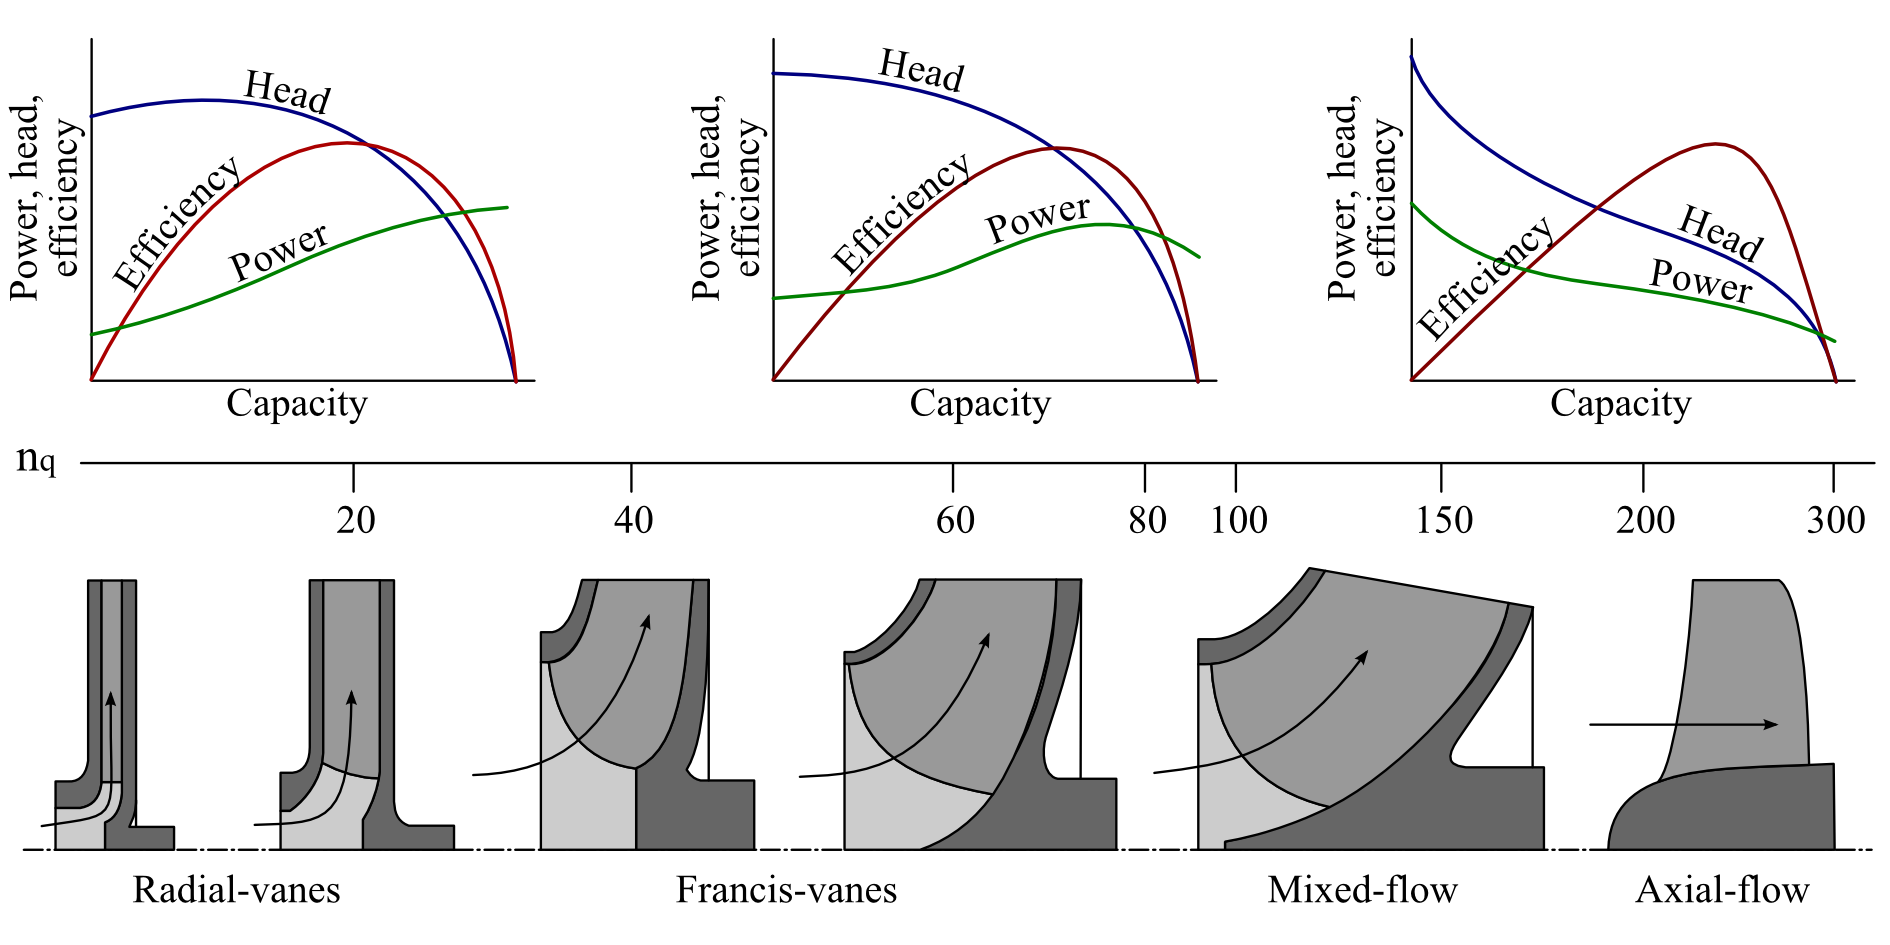
\includegraphics[width=0.8\textwidth]{figs/nq_eng.png}
\caption{\label{fig:nq}Specific speed and shape of the impeller.}
\end{center}
\end{figure}

Based on experience the available maximum efficiency can be estimated in the knowledge of $Q_{opt}$ and $n_q$ as follows

\beq
\eta_{max}=0.94-0.048 Q_{opt}^{-0.32}-0.29 \left(\log\left(\frac{n_q}{44}\right)\right)^2.
\eeq

Representing $\delta_{opt}(\sigma_{opt})$, turbomachines having good efficiency pass a narrow path. This diagram is called \emph{Cordier-diagram}. The centre of the path can be assumed with

\beq
\delta=\left(\frac{2.1}{1.41\log(\sigma)}\right)^{1.34}.
\eeq

Experience moreover shows that for a given $n_q$ estimation can be given for the ideal value of $\psi$ as follows

\beq
\psi=\left(\frac{300}{270+n_q}\right)^{9/4}.
\eeq


\subsection{Problems}

\noindent {\bf Problem \thesection.\theprob}\stepcounter{prob}

The input mechanical power of a water pump is 25 kW, the revolution number is 1440 rpm, the flow rate is 0.06 $\mathrm{m^3/s}$. The volumetric efficiency is estimated as $\eta_v=0.92$, the hydraulic efficiency is $\eta_h=0.85$, the disc friction power loss is $P'_{df}=0.9$ kW, the mechanical loss is $P'_m=1.3$ kW. Find the head and the specific speed and make a sketch of the impeller. (Solution: H=30.3m, $n_q$=27.3, the impeller is a thin radial one.)

%%%%%%%%%%%%%%%%%%%%%%%%%%%%%%%%%%%%%%%%%%%%%%%%%%%%%%%%%%%%%%%%%%%%

\vspace{1cm}
\noindent {\bf Problem \thesection.\theprob}\stepcounter{prob}

The revolution number of a pump is 1450 rpm, the head and flow rate at the best-efficiency point are 17m and 0.03 $\mathrm{m^3/s}$. Find the specific speed. Find the diameter of the impeller if, based on industrial experience, the pressure number at the best-efficiency point should be $\psi=1$. Find the flow number $\varphi$. Find the head and flow rate at 970rpm. (Solution: $n_q=30$, $D_2=240$mm, $\varphi=0.036$, $Q_{970\mathrm{rpm}}=0.02\mathrm{m^3/s}$, $H_{970\mathrm{rpm}}=7.61\mathrm{m}$) 

%%%%%%%%%%%%%%%%%%%%%%%%%%%%%%%%%%%%%%%%%%%%%%%%%%%%%%%%%%%%%%%%%

\vspace{1cm}
\noindent {\bf Problem \thesection.\theprob}\stepcounter{prob}

The head produced by a six stage pump type CR 8-60 is $H[m] = 68-0.2Q^2$, the speed of rotation is $n=2850~\frac{1}{\mathrm{min}}$. The efficiency is $\eta = 0.66-0.00731 (Q-9.5)^2$. The unit of the flow rate in the formulae is $[m3/h]$. Find the specific speed. Based on the specific speed, find the type of the impeller. Determine the input power of the water delivering pump for zero delivery $Q=0$ by extrapolation from calculated points in the range $Q = 1.5; 1; 0.5 m3/h$, and using L'Hopital's rule. (Solution: $n_q=29.9$, hence the impeller is radial; $P_{in}=1334W$.)

%%%%%%%%%%%%%%%%%%%%%%%%%%%%%%%%%%%%%%%%%%%%%%%%%%%%%%%%%%%%%%%%%

\vspace{1cm}
\begin{tcolorbox}
\noindent {\bf Problem \thesection.\theprob}\stepcounter{prob}

The characteristic curve of a pump at $n_1 = 1450/min$ rotor speed is $H_1 = 40m-40000s^2/m^5 Q^2$. Calculate 5 points of the pump-characteristic for the rotor speed $n_2 = 2900/min$ in the flow rate range $Q_2 = 0,01m^3/s-0,05m^3/s$ at $0,01 m^3/s$ intervals. According to laboratory tests the affinity law is valid in this range. Give the equation of the characteristics $H_2(Q_2)$ for the rotor speed $n_2$! (Solution: $H_2(Q_2)=160-40000Q_{2}^{2}$)
\vspace{0.2cm}

Solution:
\vspace{0.2cm}

{\bf Affinity laws:}

\begin{equation*}
	\frac{q_2}{q1}=\frac{n_2}{n_1}=2, \quad
	\frac{H_2}{H_1}=\left(\frac{n_2}{n_1}\right)^2=2^2=4
	\quad \text{and} \quad \frac{P_2}{P_1}=\left(\frac{n_2}{n1}\right)^3=2^3=8.
\end{equation*}
\vspace{0.2cm}

\begin{center}
\begin{tabular}{|c|c|c|c|c|c|c|c|}
	\hline
2.with affinity & $q_1 =q_2/2[m^3/s]$ & 0 & 0.005 & 0.01 & 0.015 & 0.02  & 0.025 \\
	\hline
3.with the caracteristic curve	& $H_1$[m] & 40 & 39 & 36 & 31 & 24 & 15 \\
	\hline
1.given & $q_2$ $[m^3/s]$ & 0 & 0.01 & 0.02 & 0.03 & 0.04 & 0.05 \\
	\hline
4.with affinity	& $H_2=4H_1$ & 160 & 156 & 144 & 124 & 96 & 60 \\
	\hline
\end{tabular}
\end{center}

\vspace{0.2cm}

{\bf Conversion of the characteristic curve analytically}

the general shape of the characteristic curve of a pump at n1 speed: $H_1=A+Bq+Cq^2$ (n this case we assumed that the characteristic curve H(q) of a pump can be described with a second degree polynomial. In reality this is a good approximation). In the present problem, the linear term (Bq) is zero.

\begin{equation*}
	H_1=A+Bq+C^2q=A+C^2q.
\end{equation*}
%(Of course, if in another task, in the case of another pump, B $\ne$ 0, the following derivation can also be performed)
%Derivation:
%
We have:
%
\begin{equation*}
	H_2=H_1\left(\frac{n_2}{n_1}\right)^2=\left(\frac{n_2}{n_1}\right)^2\left(A+C{q_1}^2\right)=1\left(\frac{n_2}{n_1}\right)^2\left[A+C{q_2}^2\left(\frac{n_1}{n_2}\right)^2\right]=A\left(\frac{n_2}{n_1}\right)^2+C{q_2}^2.
\end{equation*}
In the first step of the above derivation, the affinity for the transport height H is used, in the second the characteristic curve $H_1$ is substituted. In the third we also use the affinity for the volume flows rate q, and in the fourth we remove the parantheses from the equation. The caracteristic curve of the pump is:
%
\begin{equation*}
	H_2=A\left(\frac{n_2}{n_1}\right)^2+Cq^2=40\times\left(\frac{2920}{1460}\right)^2-40000q^2.
\end{equation*}

If the linear term $B$ is non-zero, we have
%
\begin{equation*}
	H_2=A\left(\frac{n_2}{n_1}\right)^2+B\left(\frac{n_2}{n_1}\right)q_2+C{q_2}^2.
\end{equation*}

The specific speed is
%
\begin{equation*}
	n_q=n_2 {q_{2,opt}}^{1/2}{H_{2,opt}}^{-3/4}=2920\times\frac{\sqrt{0.03}}{{124}^{3/4}}=43.04.
\end{equation*}
%
Note that this number is independent of the actual revolution number (as long as the optimal head and flow rate is properly used), which justifies its name. Finally, the characteristic curves are plotted in Figure \ref{gen_fig}

\end{tcolorbox}

\begin{figure}[ht]
\begin{center}
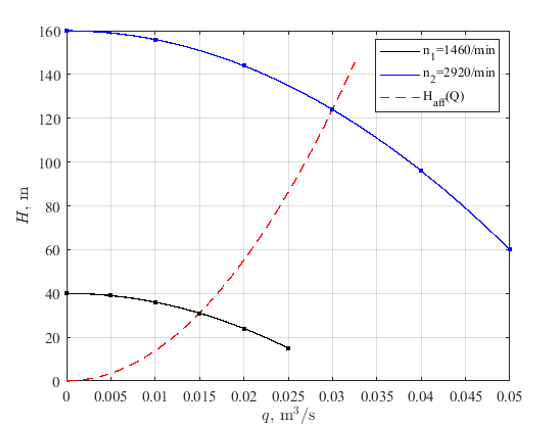
\includegraphics[scale=0.75]{figs/problem_2p4p22_aff_fig.png}
\caption{\label{gen_fig}Convert characteristic curves to other speeds}
\end{center}
\end{figure}

\vspace{1cm}

\noindent {\bf Problem \thesection.\theprob}%\stepcounter{prob} NEM ITT, AZ ABRA UTAN

Find the specific speed of the pump given by \ref{fig:PS_PerfCurves}, if the revolution number is 3000 rpm. Make a sketch of the impeller. (Solution: $n_q=92$, mixed impeller.)

\begin{figure}[!h]
\begin{center}
\centering
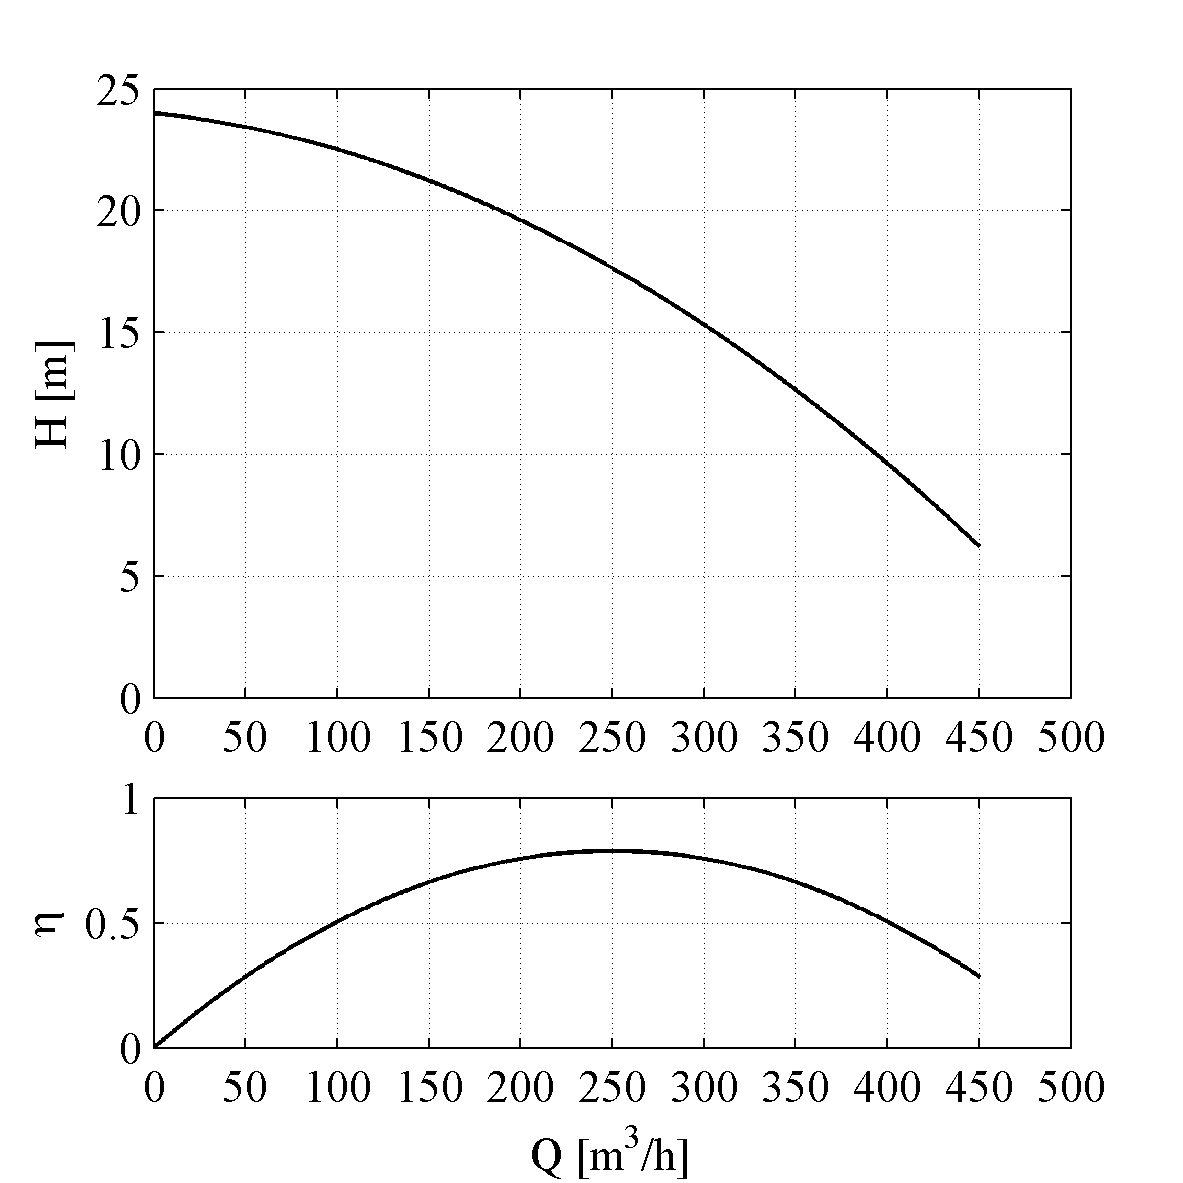
\includegraphics{Problem_solving/figs/PS_PerfCurves.png}
\caption{\label{fig:PS_PerfCurves}Performance chart for Problem \thesection.\theprob.}
\end{center}
\end{figure}
\stepcounter{prob}

%%%%%%%%%%%%%%%%%%%%%%%%%%%%%%%%%%%%%%%%%%%%%
\vspace{1cm}
\noindent {\bf Problem \thesection.\theprob}\stepcounter{prob}

The performance curve of a pump at 1450 rpm is given by $H=100-30000\,Q^2$ and the efficiency is given by $\eta=-78000\,Q^2+4500\,Q$. Find the head and flow rate of the best-efficiency point. Find the performance curve at 1740 rpm. ($H_{opt}=76$m, $Q_{opt}=0.02855\mathrm{m^3/s}$, $\eta_{max}=64.9\%$, $H_{1740\mathrm{rpm}}=144-30000\,Q^2$.)

%%%%%%%%%%%%%%%%%%%%%%%%%%%%%%%%%%%%%%%%%%%%%%%%%%%%%
\vspace{1cm}
\noindent {\bf Problem \thesection.\theprob}\stepcounter{prob}

Assuming prerotation-free flow at the inlet, find the pressure number-flow number of a radial pump with backward swept impeller at the design (optimal) point! The pump has 9 impellers, so the slip factor is approximately one $(\lambda=1)$. The blade angle at the outlet is $\beta_2=40^{\circ}$ and the flow-through width of the impeller is $9~\%$ of the outer diameter $(b_2/D_2=0.09)$. The outer diameter $D_2=200~\mathrm{mm}$, and the speed of rotation is $n=1450~\frac{1}{\mathrm{s}}$. Calculate the specific speed $(n_q)$ of the machine! At the optimal (design) operation point, the hydraulic efficiency is $\eta_h=86~\%$, the volumetric efficiency is $\eta_v=95~\%$, the flow number is $\varphi=0.12$, and the blockage ration is $\psi_2=1$. (Solution: $\psi=1.00,~H_{opt}=11.74,~Q_{opt}=0.0572,~n_q=54.68$)

\begin{tcolorbox}
Solution:

\begin{equation*}
H=\eta_h\lambda\frac{{u_2}^2}{g}\left(u_2-\frac{Q}{\eta_v\psi_2D_2\pi b_2tg\beta_2}\right)\quad \text{with}\quad  \lambda=1\quad  \text{and} \quad \psi_2=1
\end{equation*}

\begin{eqnarray}
\psi\frac{{u_2}^2}{2g}&=\frac{{u_2}^2}{2g}\eta_h\left(1-\frac{\phi\frac{{D_2}^2\pi}{4}u_2}{\eta_v u_2D_2\pi b_2tg\beta_2}\right)  \quad \rightarrow \quad\\
%\end{equation*}
%
%\begin{equation*}
\psi&=2\eta_h\left(1-\frac{1}{4\eta_v\frac{b_2}{D_2}tg\beta_2}\phi\right)=2 \cdot 0.4 \cdot \left(1-\frac{1}{4 \cdot 0.95 \cdot 0.09 \cdot tg40^oC}\phi\right)=1.72 \cdot (1-3.485 \cdot \phi)
\end{eqnarray}

\begin{equation*}
\psi_{opt}=1.72 \cdot (1-3.485 \cdot \phi_{opt})=1.72 \cdot (1-3.485 \cdot 0.12)=1,
\end{equation*}
in case of centrifugal pumps and centrifugal fans this is a common value.

\begin{equation*}
u_2=D_2\pi n=0.2 \cdot \pi \cdot \frac{1451}{60}=15.18 m/s
\end{equation*}

\begin{equation*}
H_{opt}=\psi_{opt}\frac{{u_2}^2}{2g}=1 \times \frac{15.18^2}{2 \cdot 9.81}=11.74m
\quad  \text{and}  \quad
Q_{opt}=\phi_{opt}\frac{{D_2}^2\pi}{4}=0.12 \cdot \frac{0.2^2 \pi }{4} 15.18=0.0572 m^3/s 
\end{equation*}

From whic we have
%
\begin{equation*}
n_q=n\frac{\sqrt{Q{opt}}}{{H_{opt}}^{\frac{3}{4}}}=1450 \cdot \frac{\sqrt{0.0572}}{{11.74}^\frac{3}{4}}=55
\end{equation*}
\end{tcolorbox}

%%%%%%%%%%%%%%%%%%%%%%%%%%%%%%%%%%%%%%%%%%%%%%%%%%%%%
%\vspace{1cm}
%\noindent {\bf Problem \thesection.\theprob}\stepcounter{prob}

%The inner $(i)$ diameter of an axial pumps impeller is $D_i=250~\mathrm{mm}$, and the outer $(o)$ diameter is $D_o=400\mathrm{mm}$ The speed of rotation $n=1470~\frac{1}{\mathrm{min}}$. At the inlet, prerotation-free flow can be assumed $(c_{1,u}=0)$. The hydraulic efficiency $\eta_h=0.85$, the head of the pump $H=6\mathrm{m}$, and the volumetric flow rate is $Q=0.36~\frac{\mathrm{m^3}}{\mathrm{s}}$. The specific work of the machine is approximately constant along the impellers, meaning $Y = c_{2,u}(r)u_2(r) = c_{2,u,i}u_{2,i} = c_{2,u,o}u_{2,o} = \mathrm{const.}$. Calculate the blade angles at the base of the blade $(\beta_{1,i}=?,~\beta_{2,i}=?)$, and at the tip of the blade $(\beta_{1,o}=?,~\beta_{2,o}=?)$! (Solution: $\beta_{1,i}=13.73,~\beta_{2,i}=16.7, (\beta_{1,o}=8.7,~\beta_{2,o}=9.4$)

\clearpage
\section{Forces on the impeller}

%\subsection{Radial force}
%
%\fbox{TODO}

\subsection{Axial force}
\note{Axial Force is written by Weber Richard}

The axial force results from two components:
\begin{itemize}
\item Momentum force
\item Pressure distribution on the hub(back of the impeller) and shroud(front of the impeller).
\end{itemize}

The overall axial force is
%
\beq
F_{ax}=F_{hub}-F_{shroud}+F_{impulse}+ \underbrace{mg,}_{\text{in case of vertical impeller}}
\eeq
%
and its direction is towards the suction side (the axial force tries to 'pull down' the impeller from the shaft).
The impulse force is
\beq
F_{impulse}=\dot{m} v =  \underbrace{\rho Q}_{\dot{m}}  \underbrace{\frac{Q}{A_1}}_{c_{in}} = \rho \frac{Q^2}{A_1}.
\eeq
The force on the hub and the shroud can be calculated from the pressure distribution along the impeller. 

\begin{figure}[!h]
\begin{center}
\centering
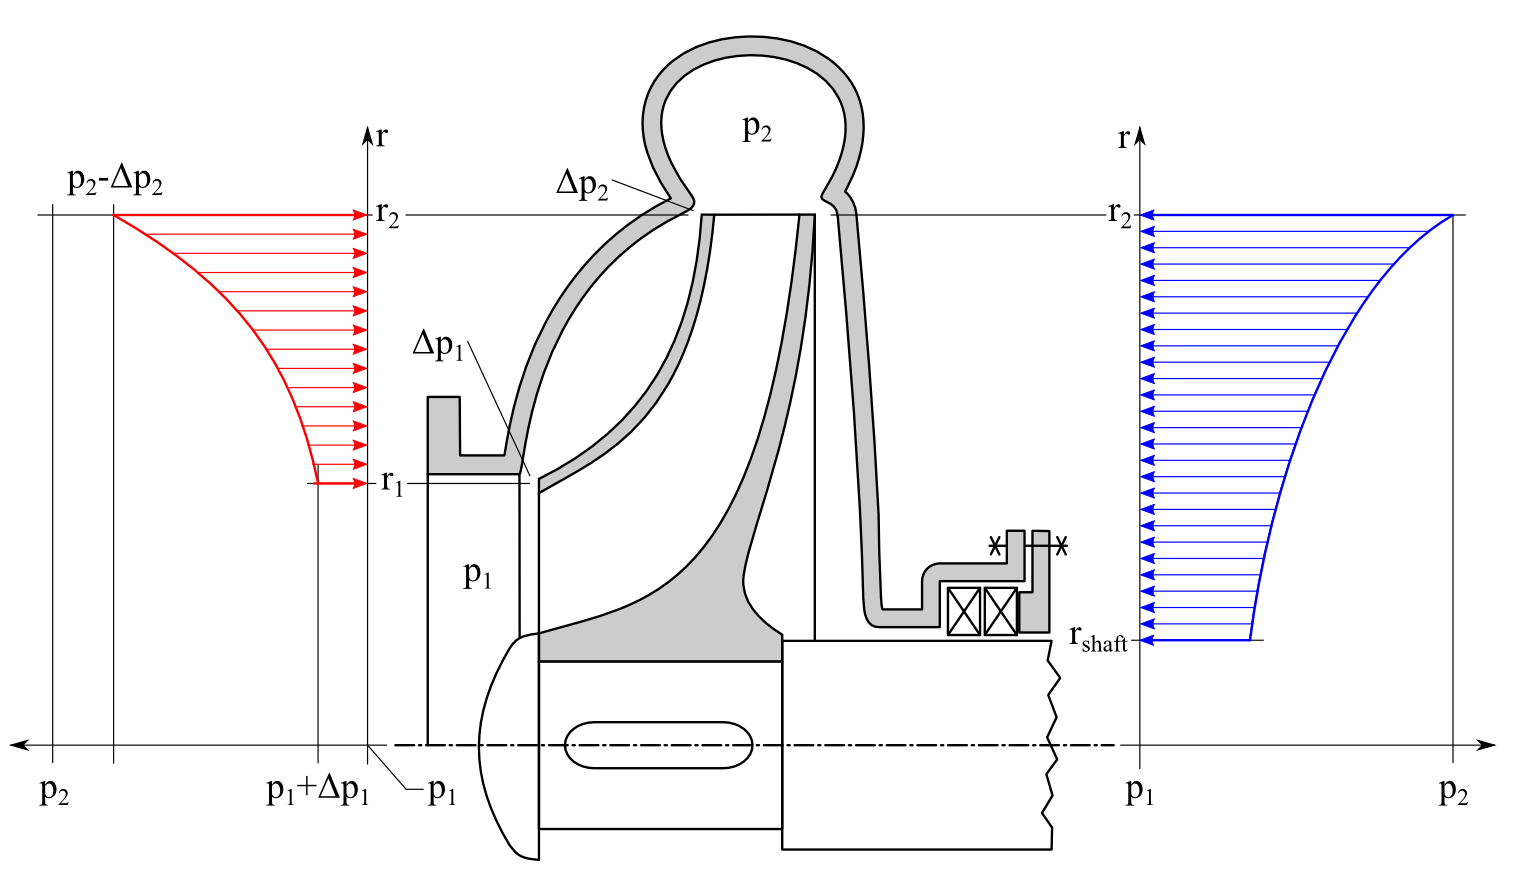
\includegraphics{figs/AxialForces.png}
\caption{\label{fig:ax_force}Pressure distribution on the hub.}
\end{center}
\end{figure}

In general for a rotating frame the pressure distribution is 
\beq
p(r) =  K + \frac{\rho}{2} (r \omega_f)^2,
\eeq
where $K$ is a constant and $\omega_f$ is the angular velocity of the fluid.

$K$ can be calculated from the boundary condition. Since the pressure exactly known at the end of the impeller ($r=r_2$). For the hub this is
\beq
p_h(r_2)=p_2 \quad \rightarrow \quad p_h(r)=p_2-\frac{\rho}{2}\omega_f^2\left( r_2^2-r^2\right).
\eeq
In case of the shroud a pressure drop ($\Delta p_2$) is reducing the pressure at the boundary:
\beq
p_s(r_2)=p_2-\Delta p_2 \quad \rightarrow \quad p_s(r)=p_2-\Delta p_2-\frac{\rho}{2}\omega_f^2\left( r_2^2-r^2\right).
\eeq
The forces can be evaluated as the definite integral of the pressure distribution.
The axial force becomes on the hub (back of the impeller):
\begin{eqnarray}
F_{hub} &=&\int_{r_s}^{r_2} 2 r \pi p_h(r) dr = 2 \pi \int_{r_s}^{r_2} p_2 r - \frac{\rho}{2} \omega_f^2 \left(r_2^2 r-r^3\right)dr = \nonumber \\
 &=& 2 \pi \left[ p_2 \frac{r_2^2 - r_s^2}{2} - \frac{\rho}{2} \omega_f^2 \left( r_2^2 \frac{r_2^2-r_s^2}{2} - \frac{r_2^4-r_s^4}{4} \right) \right] = \nonumber\\
&=& 2 \pi \frac{r_2^2-r_s^2}{4} \left[ p_2 - \frac{\rho}{2} \omega_f^2 \left( r_2^2 - \frac{r_2^2-r_s^2}{2} \right) \right],
\end{eqnarray}
finally
\begin{equation}
F_{hub}  =\left( r_2^2-r_s^2\right)\pi \left( p_2-\frac{\rho}{2}\omega_f^2\frac{r_2^2-r_s^2}{2}\right).
\end{equation}
%
A similar result is obtained for the shroud (front of the impeller) with replacing $r_s$ by $r_1$:
\begin{equation}
F_{shroud} = \left( r_2^2-r_1^2\right)\pi \left( p_2 - \Delta p_2-\frac{\rho}{2}\omega_f^2\frac{r_2^2-r_1^2}{2}\right).
\end{equation}

\section{Problems}

\noindent {\bf Problem \thesection.\theprob}\stepcounter{prob}

Find the axial force on the back of the impeller, whose outer diameter is $D_2=300$mm, the shaft diameter is $D_s=50$mm, the outlet pressure is $2.3$bar and the revolution number is 1470rpm. The average angular velocity of the fluid is 85\% of that of the impeller. (Solution: $F=9.36$kN)

%%%%%%%%%%%%%%%%%%%%%%%%%%%%%%%%%%%%%%%%%%%%%%%%%%%%

\vspace{1cm}
\noindent {\bf Problem \thesection.\theprob}\stepcounter{prob}

Calculate the axial force acting on the supporting disc of a pump impeller of $280 mm$ diameter if the pressure at the impeller exit is $2 bar$. The hub diameter is $40 mm$. There is no leakage flow through the gap between the rotor supporting disc and the casing. The rotor speed is $1440/min$. The angular velocity of the circulating water is half of that of the rotor. Find the formula of pressure distribution as a function of the radial coordinate! Draw the cross section of the impeller and the axial pressure force! (Solution: $p(r)(\mathrm{Pa}) = 1.443\cdot 10^5 + 2.842\cdot 10^6 \cdot r^2$, $F_{ax} = 10418~\mathrm{N}$)

\section{Cavitation}
\note{written by Weber Richard}

\begin{figure}[!h]
	\begin{center}
	\centering
	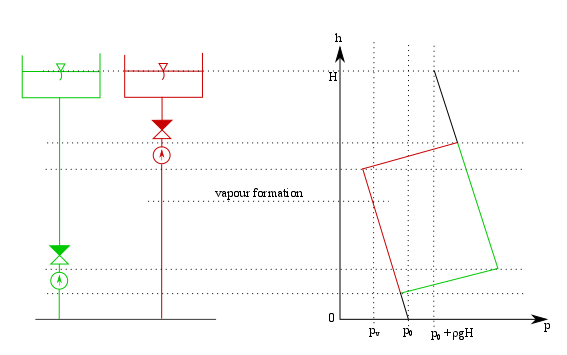
\includegraphics[width=13cm]{figs/cavitation.png}
	\caption{\label{fig:cavitation}Representation of the cavitation.}
	\end{center}
\end{figure}

Two similar arrangement can be seen on left side of Figure \ref{fig:cavitation}. The only difference is the height of the pump, although this cause major deviation in the pressure distribution along the pipe line as it can be observed on the right side of the Figure. In the worst cases the pressure can be below the saturation vapour pressure which means locally the vapour bubbles are appearing. This is called cavitation. The vapour pressure is usually a function of the temperature, e.g.  for water:

\begin{center}
	\begin{tabular}{lcccccc}
	$t[C]$ & 10 & 20 & 40 & 60 & 80 & 100 \\
	$p_v [bar]$ & 0.012 & 0.02 & 0.07 & 0.2 & 0.47 & 1\\
	\end{tabular}
\end{center}

There could be three major consequences of the cavitation:
\begin{itemize}
\item Increased noise among vibration,
\item Drastic decrease in hydraulic performance curve: $H-Q$,
\item Damage of the impeller, see Figure \ref{fig:cavitation_damage}.
\end{itemize}
\begin{figure}[!h]
	\begin{center}
	\centering
	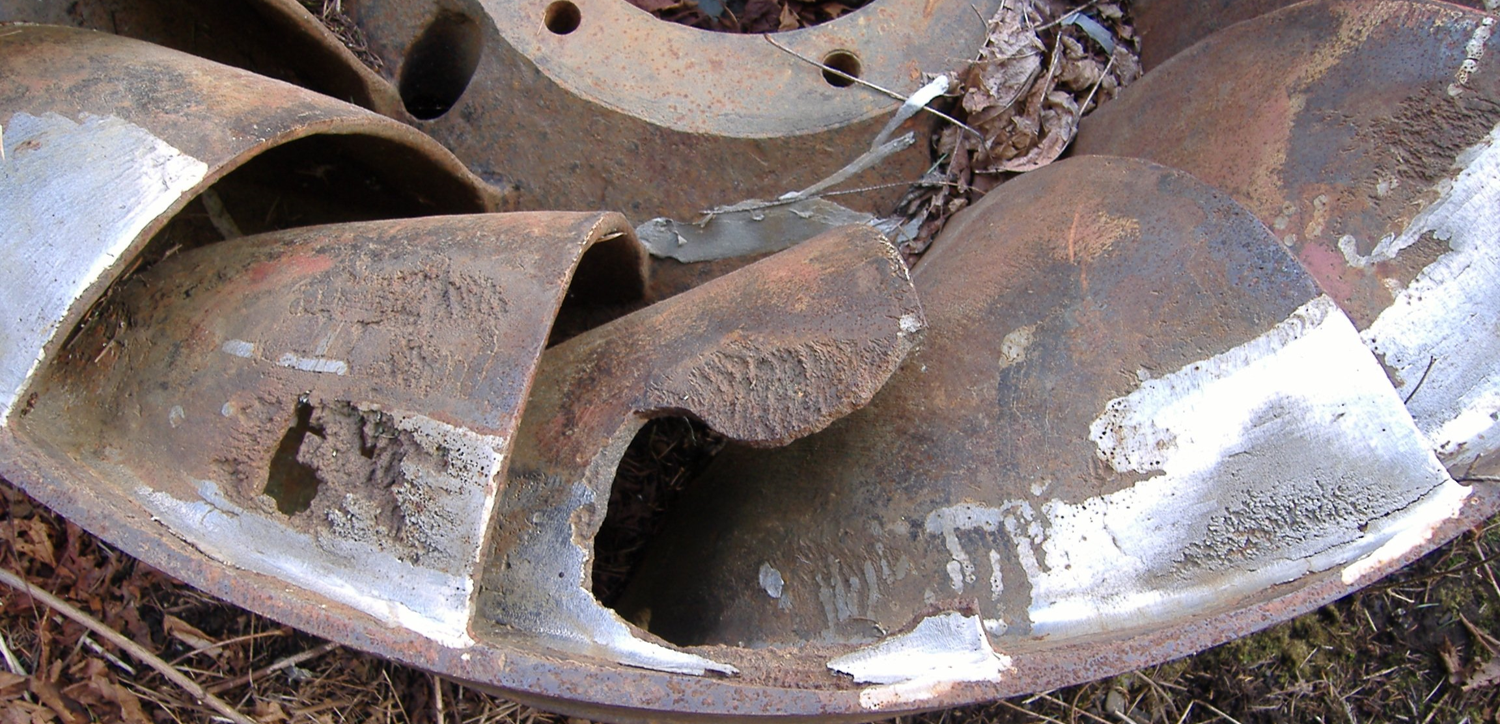
\includegraphics[width=13cm]{figs/cavitation_damage.png}
	\caption{\label{fig:cavitation_damage}Illustration of the cavitation damage in pumps.}
	\end{center}
\end{figure}

\newpage
\subsection{Net Positive Suction Head (NPSH)}

To avoid cavitation it is not sufficient to ensure that the pressure at the suction side is larger than the vapour pressure ($p_s > p_v$). Since  inside the pump there is a complex flow, therefore it is possible to have $p<p_s$ locally where the velocity is large enough. Ensuring the operational work without cavitation the $\mathit{NPSH}$ has to be defined. It is convenient to split the absolute pressure at the pressure side $p_s$ into two parts: $p_v$ vapour pressure plus the part above that, deonted by $\rho g \times NPSH$:
%
\begin{equation}
p_s = p_v + \rho g \times \underbrace{\mathit{NPSH}}_{\text{Net Positive Suction Head}}
\end{equation}
%
this way, the NPSH value gives the net "standby" pressure \emph{above} the vapour pressure that is available before cavitation occurs. 

\begin{figure}[!h]
	\begin{center}
	\centering
	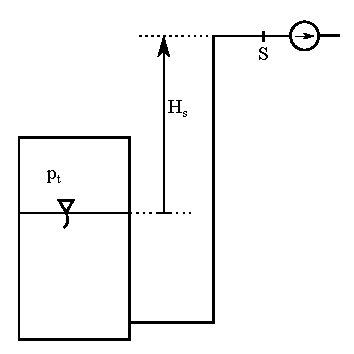
\includegraphics[width=6cm]{figs/NPSH.pdf}
	\caption{\label{fig:NPSH}Representation of the NPSH.}
	\end{center}
\end{figure}

There are two different $\mathit{NPSH}$ values: available ($\mathit{NPSH}_a$) and the required ($\mathit{NPSH}_r$):

\begin{itemize} 
	\item {\bf The available $\mathit{NPSH}_a$} is a {\bf property of the hydraulic system} (geometry, loss coefficients etc. of the pipelines and tanks) and can be evaluated as
\begin{eqnarray}
\mathit{NPSH}_a = \frac{p_t - p_v(T)}{\rho g} - H_s - h'(Q),
\end{eqnarray}
where the $h'(Q)$ represents the frictional losses at the suction-side pipeline (see later in Section \ref{sec:frictionallosses}). 
%
\item {\bf The required $\mathit{NPSH}_r$} value can be found {\bf in the catalogue of the pump}. It is usually depending on the volume flow rate similarly to the head. 
\end{itemize}

The condition for avoiding the cavity is that the available $\mathit{NPSH}$ must be larger than the required $\mathit{NPSH}$, mathematically:
\begin{eqnarray}
\mathit{NPSH}_a > \mathit{NPSH}_r \hspace{1cm} \Longleftrightarrow \hspace{1cm} \text{\textbf{no cavitation}}
\end{eqnarray}

\subsection{Problems}

\vspace{1cm}
\noindent {\bf Problem \thesection.\theprob}\stepcounter{prob}

A pump delivers water from a low-pressure steam boiler as shown in the figure below. Calculate the required geodetic height of the reservoir to avoid cavitation! The pipeline losses are to be taken into account.

\begin{tabular}{cc}
    \begin{minipage}{6cm}
	\begin{center}
	    \resizebox{5cm}{!}{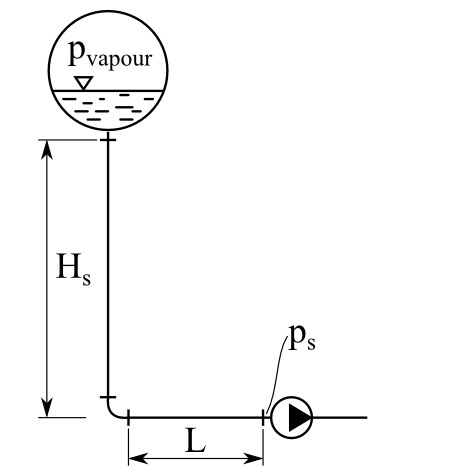
\includegraphics{Problem_solving/figs/PS_NPSH_figure2.png}}\\
	\end{center}
    \end{minipage}
& 

\begin{minipage}{9cm}
\begin{itemize}
\item mass flow rate: $\dot m=27 [kg/s]$, density of the hot water: $\rho=983 [kg/m^3]$
\item pipe: $L=10[m]$, $d=100[mm]$, $\lambda=0.02$ and the sum of loss factors is $\zeta=5$
\item pump: $H[m]=82-4800\,Q^2$, $\mathit{NPSH}[m]=1.6+1360\, Q^2$
\end{itemize}

\emph{Solution:} 

It's easy to calculate that\\
$Q=\dot m/ \rho=0.02747 [m^3/s]$ \\ 
$c_s=Q/A=3.5[m/s]$\\
$H=82-4800 \times 0.02747^2=78.38[m]$\\ 
$\mathit{NPSH}=1.6+1360 \times 0.02747^2=2.626[m]$ 

\end{minipage}
\end{tabular}

\vspace{0.5cm}

Bernoulli's equation between a surface point in the tank and the suction side of the pump reads:

\begin{equation*}
\frac{p_t}{\rho g} + \frac{0^2}{\rho g}+H_s\,=\,\frac{p_s}{\rho g} + \frac{c_s^2}{\rho g}+0+h'_{pipeline}
\end{equation*}

From the suction side of the pump to the impeller we have:

\begin{equation*}
\frac{p_s}{\rho g} + \frac{c_s^2}{2 g}\,=\,\frac{p_{vapour}}{\rho g} + e_s + \mathit{NPSH}
\end{equation*}

(Note that $e_s=0$ as the configuration is horizontal.) Putting the above two equations together, we have

\begin{equation*}
\mathbf{H_s} =-\frac{p_t-p_{vapour}}{\rho g} + h'_{pipe} + \mathit{NPSH}, \quad \text{where} \quad h'_{pipe} = \frac{c_s^2}{2g}\left( \lambda \frac{\mathbf{H_s}+L}{d}+\zeta \right),
\end{equation*}

thus,

\begin{equation*}
H_s =\left( 1-\frac{c_s^2}{2g} \frac{\lambda}{d} \right)^{-1} \left[ \mathit{NPSH} + \frac{c_s^2}{2g} \left( \frac{\lambda L}{d}+\zeta \right) \right]=\dots=8.116[m]
\end{equation*}

Thoma's cavitation coefficient is $\sigma=\mathit{NPSH}/H=0.03355[-]$.

\vspace{1cm}
\noindent {\bf Problem \thesection.\theprob}\stepcounter{prob}

Calculate the required pipe diameter to avoid cavitation, if the pump delivers $Q=30\,\mathrm{dm^3/s}$ water from a closed tank, where the pressure (above the water level) is $p=40\,\mathrm{kPa}$. The equivalent pipe length on the suction side is $5m$, the friction coefficient is $\lambda=0.02$, the suction flange of the pump is $3\,\mathrm{m}$ below the water level. The vapour pressure at the water temperature is $2.8\,\mathrm{kPa}$. The required net positive suction head is $\mathit{NPSH}_r=3.2\,\mathrm{m}$. (The standard pipe diameter series is: DN 40, 50, 65, 80, 90)

\noindent Solution:

\noindent The sketch of the installation is shown in Figure~\ref{fig:NPSH_figure1}

\begin{figure}[ht]
\centering
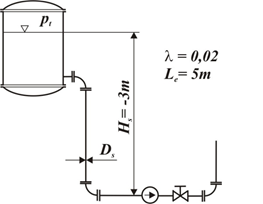
\includegraphics[width=0.37\textwidth]{Problem_solving/figs/PS_NPSH_figure1.png}
\caption{\label{fig:NPSH_figure1}Installation of the apparatus.}
\end{figure}

\begin{itemize}
\item $\mathit{NPSH}_a=\frac{p_t-p_v}{\rho g}-H_s-h'_s\quad\rightarrow h'_s=\frac{p_t-p_v}{\rho g}-H_s-\mathit{NPSH}_r$
\item $h'_s=\lambda \frac{L_e}{D_s}\frac{c^2_s}{2g}=\lambda \frac{L_e}{D_s}\frac{8Q^2}{D^4_s g \pi^2}$
\item $D_s=0.073m\rightarrow D_s=80\,\mathrm{mm}$
\end{itemize}

\vspace{1cm}
\noindent {\bf Problem \thesection.\theprob}\stepcounter{prob}

Find the required suction side height of the pump that conveys water from an open surface reservoir at $Q=180m^3/h$ flow rate the head is $H=30m$ the required net positive suction head $\mathit{NPSH}_r=5.03m$. The temperature of the water is $T=23^\circ$ the ambient pressure is $p_0=1023mbar$. The hydraulic loss of the suction side pipe can be calculated from $h'_s=652[s^2/m^5]Q^2$ while the vapour pressure $p_v (\mathrm{kPA})=1.704+0.107(t-15)+0.004(t-15)^2$. Find the Thoma cavitation number. (Solution: $H_s=3.481m$, $\sigma=0.1677$)



\clearpage
